

\documentclass[8pt, usepdftitle=false]{beamer}
% \imput{../common/beamerthemesimple}
\usetheme{simple}


  \usepackage{xcolor}
  \definecolor{olive}{rgb}{0.3, 0.4, .1}
  \setbeamercolor{itemize/enumerate body}{fg=black}
  \setbeamercolor{title}{fg = green!30!black}
  \setbeamercolor{frametitle}{fg = gray!70!black, bg = white}


% \usepackage{lmodern}
\usepackage[scale = 2]{ccicons}
\usepackage[export]{adjustbox}
\usepackage{amsmath, amsthm, amssymb}
\usepackage{amsfonts}
\usepackage{mathtools}

\usepackage[justification=raggedright,width=\linewidth]{caption}
\usepackage{tikz} 


\usepackage{setspace}

\setbeamertemplate{title page}[default][right,colsep=-4bp,rounded=true,shadow=\beamer@themerounded@shadow]

\setbeamertemplate{caption}[numbered]


%% Options

\setbeamercolor{alerted text}{fg=blue}
\setbeamertemplate{alerted text begin}{\itshape}
\setbeamertemplate{alerted text end}{}

\newenvironment<>{varblock}[2][\textwidth]{%
    \setlength{\textwidth}{#1}
    \begin{actionenv}#3%
        \def\insertblocktitle{\underline{#2}}%
        \par%
        \usebeamertemplate{block begin}}
        {\par%
        \usebeamertemplate{block end}%
    \end{actionenv}}

\setbeamertemplate{blocks}[rounded][shadow=true]
\setbeamercolor{block title}{fg=black,bg=gray!20!white}
\setbeamercolor{block body}{fg=black,bg=gray!10!white}




%% Theorem

% \newtheorem{theorem}{Theorem}

%% Bangla tex


\usepackage{polyglossia}
\setotherlanguage[numerals=Devanagari]{bengali}
\setmainlanguage{english}
\newfontfamily\bengalifont[Script=Bengali]{Akaash}


%% tikx

\usepackage{tikz}
\usetikzlibrary{calc,trees,positioning,arrows,fit,shapes,calc}





\newcommand\blfootnote[1]{%
  \begingroup
  \renewcommand\thefootnote{}\footnote{#1}%
  \addtocounter{footnote}{-1}%
  \endgroup
}



\newcommand\Permute[2][^n]{\prescript{#1\mkern-2.5mu}{}P_{#2}}
\newcommand\Combine[2][^n]{\prescript{#1\mkern-0.5mu}{}C_{#2}}


\renewcommand*{\thefootnote}{\fnsymbol{footnote}}


\usepackage{flexisym}
\usepackage{breqn}

\usepackage[T1]{fontenc}

% \usepackage{mathpazo}
% \renewcommand{\rmdefault}{put}

% \usepackage{fourier} 
% Only use the math font of mathpazo
% \let\temp\rmdefault
% \usepackage{mathpazo}
% \let\rmdefault\temp
% \renewcommand{\rmdefault}{put}


% \usepackage[hyphens]{url}


  % \usefonttheme{professionalfonts} % using non standard fonts for beamer
  % \usefonttheme{serif} % default family is serif

  % \usepackage{gentium}
  \usepackage{multicol}
  \usepackage{mathpazo}



% \renewcommand{\familydefault}{\sfdefault}  


  % color brackets
  \makeatletter
  \newcount\bracketnum
  \newcommand\makecolorlist[1]{%
      \bracketnum0\relax
      \makecolorlist@#1,.%
      \bracketnum0\relax
  }
  \def\makecolorlist@#1,{%
      \advance\bracketnum1\relax
      \expandafter\def\csname bracketcolor\the\bracketnum\endcsname{\color{#1}}%
      \@ifnextchar.{\@gobble}{\makecolorlist@}%
  }
  \let\oldleft\left
  \let\oldright\right
  \def\left#1{%
      \global\advance\bracketnum1\relax 
      \colorlet{temp}{.}%
      \csname bracketcolor\the\bracketnum\endcsname
      \oldleft#1%
      \color{temp}%
  }
  \def\right#1{%
      \colorlet{temp}{.}%
      \csname bracketcolor\the\bracketnum\endcsname
      \oldright#1%
      \global\advance\bracketnum-1\relax
      \color{temp}%
  }
  \makeatother


  \makecolorlist{black,blue,red}






\setbeamertemplate{section in toc}{%
  {\color{firstcolor}\inserttocsectionnumber.}~\inserttocsection}
\setbeamercolor{subsection in toc}{bg=white,fg=black}
\setbeamertemplate{subsection in toc}{%
  \hspace{1.2em}{\color{firstcolor}\rule[0.3ex]{3pt}{3pt}}~\inserttocsubsection\par}


\setbeamerfont{section in toc}{size=\fontsize{6}{8}\selectfont}
\setbeamerfont{subsection in toc}{size=\fontsize{6}{8}\selectfont}
\setbeamerfont{subsection in toc shaded}{size=\fontsize{6}{8}\selectfont}


\makeatletter
\patchcmd{\beamer@sectionintoc}{\vskip1.5em}{\vskip0.5em}{}{}
\makeatother






  \usepackage{twemojis}
  \usepackage{fontspec}
  \usepackage{tikzsymbols}
  \newfontfamily\DejaSans{DejaVu Sans}

% for R
\usepackage[fixed]{fontawesome5}


\setbeamercolor{emph}{fg=red}
\renewcommand<>{\emph}[1]{%
  {\color{purple}\only#2{\rm\itshape}#1}%
}

\setbeamertemplate{frametitle continuation}{}


\usepackage[round,  maxcitenames=10, mincitenames=11]{natbib}
\setlength{\bibhang}{0pt}
\renewcommand{\bibsection}{}
\usepackage{fancybox}


\setbeamertemplate{section page}
{
    \begingroup
    \begin{beamercolorbox}[sep=12pt,center]{section title}
        \usebeamerfont{section title}\insertsection\par
    \end{beamercolorbox}
    \endgroup
}

\setbeamertemplate{subsection page}
{
    \begingroup
    \begin{beamercolorbox}[sep=12pt,center]{section title}
        \usebeamerfont{section title}\insertsection\par
    \end{beamercolorbox}
    \vspace*{-1pt}
    \begin{beamercolorbox}[sep=8pt,center]{subsection title}
        \usebeamerfont{subsection title}\insertsubsection\par
    \end{beamercolorbox}
    \endgroup
}



\newcommand\Var[1]{\mathbb{V}\mathrm{ar}{#1}}



\renewcommand{\emph}[1]{%
{\rm\itshape{\color{purple}#1}}%
}

\renewcommand{\alert}[1]{%
{\rm\itshape{\color{blue}#1}}%
}

\usepackage{hyperref}
\hypersetup{
pdftitle={Ch1 - Descriptive Statistics},
  pdfsubject={},
  pdfkeywords= {Statistics},
pdfauthor={Hossain},
  pdfborder={0 0 0},
colorlinks,
citecolor=blue,
linkcolor=green!40!black,
breaklinks=true}

\usepackage{cleveref}




\newcounter{mytheorem}
\renewcommand{\themytheorem}{1.\arabic{mytheorem}}
\newcommand{\Thm}[1]{\refstepcounter{mytheorem}\textbf{#1\color{blue}\themytheorem}:}




%================ Give the title ============================##

\title{\LARGE Ch1 - Descriptive Statistics}

\subtitle{{\fontsize{10}{10}\selectfont\color{gray!50!balck} 
(\rm \itshape Graphical and Numerical Methods for Summarizing Data)}
\\\vspace*{.2cm} \scshape ECO 104 - Statistics For Business and Economics - I}

\author{Shaikh Tanvir Hossain\vspace*{-.4cm}}
\institute{ East West University, Dhaka\\  \today}
\date{\vspace{-5pt}}


% \titlegraphic{\includegraphics[width=300,height=.5\textheight]{Images/EWU.png}}

% \setbeamertemplate{background}{\tikz[overlay,remember picture]\node[opacity=0.90]at (current page){\includegraphics[width=.5\textwidth,left]{EWU.png}};}




\begin{document}

% input the outline 

\begin{frame}[plain,noframenumbering] 
    \maketitle
\end{frame}
\setbeamertemplate{background}{}
\setlength{\abovedisplayskip}{-2pt}
\setlength{\belowdisplayskip}{4pt}
\setlength{\abovedisplayshortskip}{-3pt}
\setlength{\belowdisplayshortskip}{4pt}


\AtBeginSection[]
{
    \begin{frame}[plain, allowframebreaks]
\setstretch{.1}

        \setlength{\parskip}{1ex}
            \tableofcontents[sections={1-7}, 
            currentsubsection, 
            sectionstyle=show/hide, 
            sectionstyle=show/shaded, 
            ]
    \end{frame}
}


% Hide progress bar and footline on titlepage
\begin{frame}{Outline}
 \vspace*{.2cm}

\begin{center}
\begin{minipage}{10cm}
  \begin{alertblock}{Outline}
  \setstretch{.1}
   \setlength{\parskip}{1ex}
  \tableofcontents[sections={1-10}]
  %   \framebreak
  % \tableofcontents[sections={2}]
\end{alertblock}
\end{minipage}
\end{center}


\end{frame}




\section{What is Statistics}

\begin{frame}{What is Statistics?}

\begin{itemize}
\item In one line perhaps we can say .... 

\begin{center}
  \alert{Statistics is the language which we use to collect, analyze and interpret a data}.
\end{center}

\item What is data? 

\begin{center}
  \alert{Data is a set of information presented in a systematic way.}
\end{center}

\item In this world, the use of data is almost everywhere, and often it happens so fast that we don't even realize it. 


\begin{figure}
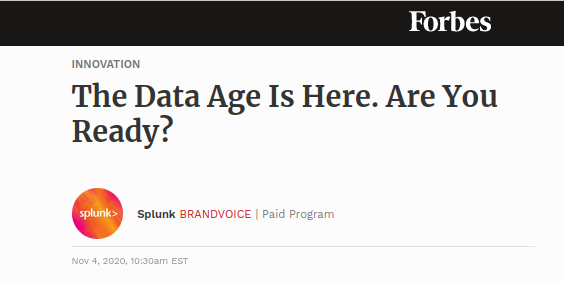
\includegraphics[scale = .4]{Images/data_age.png}
\caption{A title of an article of the Forbes magazine, November 4, 2020}
\end{figure}


\item Let's see some real life examples.

\end{itemize}

\end{frame}


%--------------------------------------------------------------------------------

\begin{frame}{What is Statistics?}

\begin{itemize}
\item
  \textbf{Location data:} Think about you are driving a car with your
  friend. Then if you are using GPS, Google collects data about where
  are you, where you going and and how much time it takes to reach the destination. Then Google uses this data to give you a \emph{prediction} about the traffic. Just open Google map, and you will probably see it.
\end{itemize}

\begin{figure}
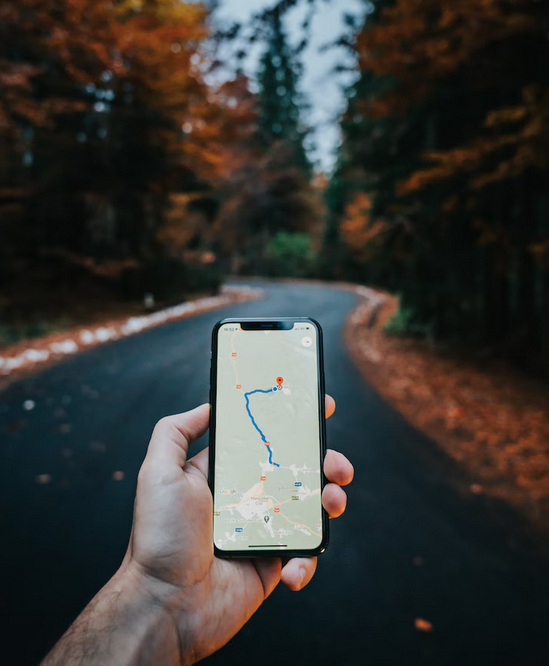
\includegraphics[scale = .2]{Images/GPS_data.png}
\caption{GPS trackers}
\end{figure}
\end{frame}


\begin{frame}{What is Statistics?}
\begin{itemize}
\item
  \textbf{Browsing data:} Google and Facebook collects many information
  when you are on your web browser searching for different things. These are all data. Google continuously collects this and then shows you contents that you might find interesting and useful. Sometimes they also sell this data to other companies (e.g., as  a part of marketing). Interestingly Google also shares different search patterns across the world, look at google trend website \footnote[frame]{\url{https://trends.google.com/trends/?geo=BD}}.
\end{itemize}

  \vspace*{.1cm}
  \begin{figure}
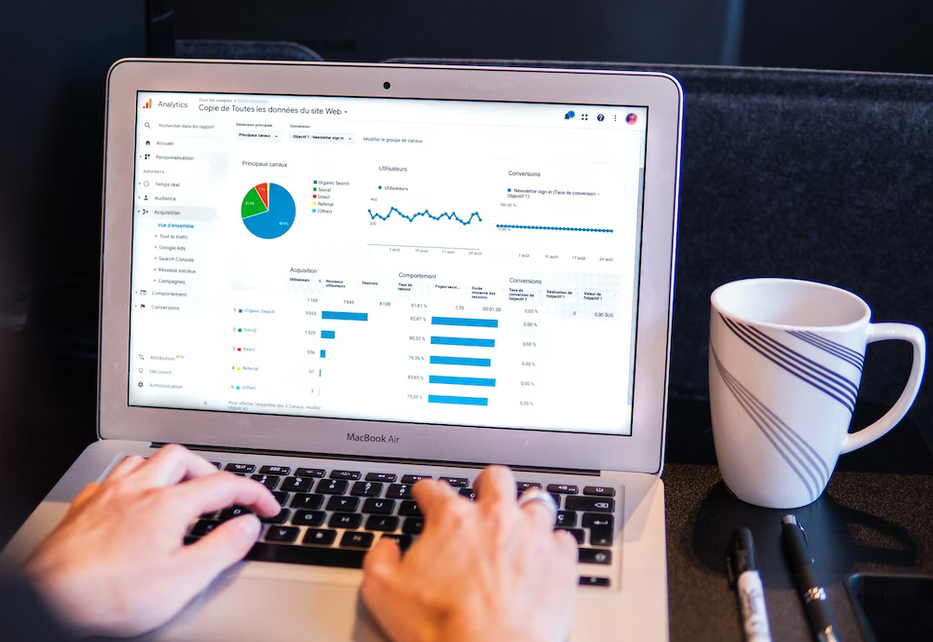
\includegraphics[scale = .2]{Images/Browsing_data.png}
\caption{Browsing data}
\end{figure}


\end{frame}


%-----------------------------------------------------------
\begin{frame}{What is Statistics?}
\begin{itemize}
\item

  \textbf{Household Surveys:} Sometimes Government or other research organizations collects important information from families or households using surveys.  This is known as \alert{household surveys}. This has information about family income,
  expenditure, education levels and many more. With this data we can get many useful information, for example average income or expenditures of different families in  Bangladesh. 

\end{itemize}
  \vspace*{-.2cm}
  \begin{figure}
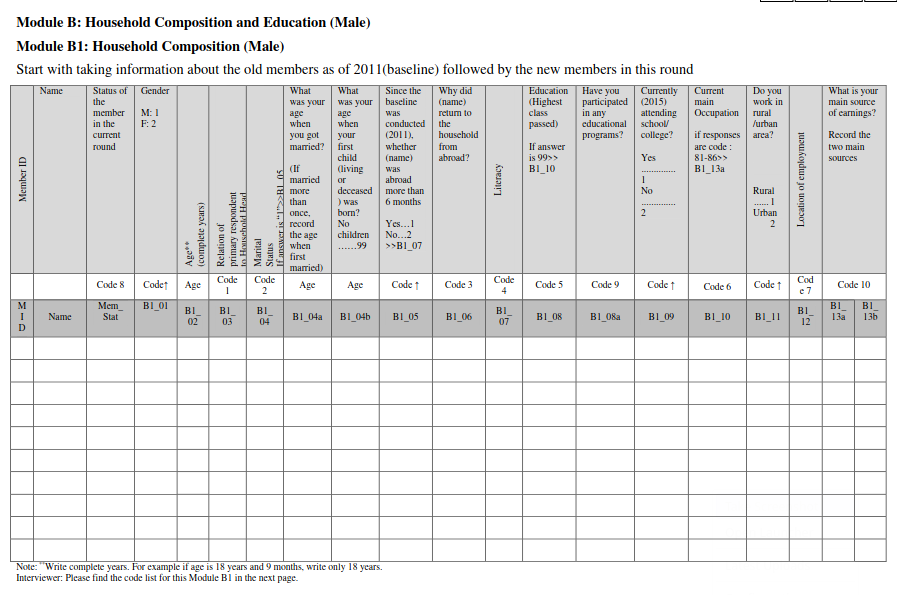
\includegraphics[scale = .3]{Images/survey_data.png}
\vspace*{-.3cm}
\caption{A page from the questionnaire of the Bangladesh Integrated Household Survey (BIHS) 2015, IFPRI}
\end{figure}




\end{frame}


%-----------------------------------------------------------


%-----------------------------------------------------------
\begin{frame}{What is Statistics?}
\begin{itemize}


\item
  \textbf{Weather Forecasts:} We all know about whether forecasts. Now this is also an application of Statistics. Whether it is going to be raining tomorrow or not, we can try to predict this using historical weather data in the specific location. 
\item
  \textbf{Financial data:} If you are an expert with financial data, perhaps you might get very rich! Actually it's not that simple. but it's true that financial data is possibly the earning source of many people.

  \item \textbf{Data analyst in companies:} Many companies are now looking for good data analysts. You might have heard about ``Machine Learning'' or ``Data Science''\footnote[frame]{If not, just google them.}. Usually any company has lots of data about its different activities, and if we can analyze these data properly, this might be very beneficial for the company, because companies can use them for different tasks, for example maximizing the sales, minimizing the costs, planning, and perhaps many more.


\end{itemize}
\end{frame}

%-----------------------------------------------------------


%-----------------------------------------------------------
\begin{frame}{What is Statistics?}

\begin{figure}
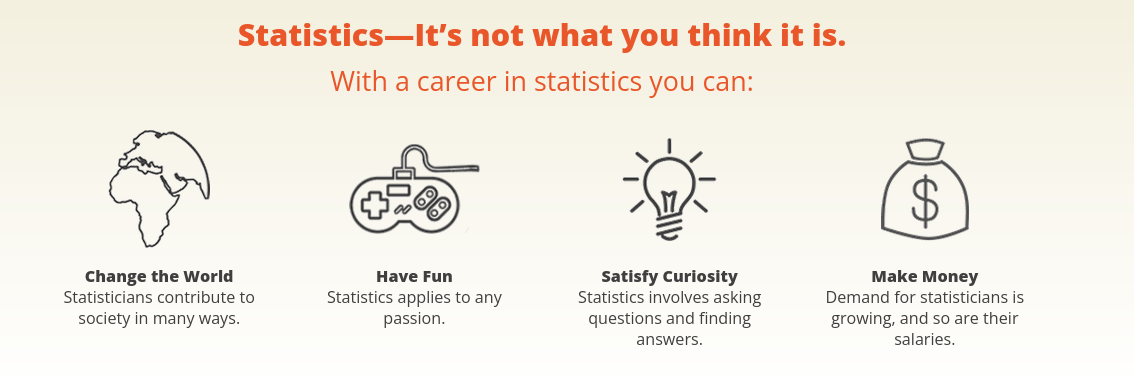
\includegraphics[scale = .3]{Images/statistics_career.png}
\caption{About the Statistics Career, taken from \url{https://thisisstatistics.org/}}
\end{figure}


\end{frame}





%-----------------------------------------------------------
\begin{frame}{What is Statistics?}
\begin{itemize}

  \item So now you got some idea about different type of data sets, and the work of Statistics is to analyze and extract useful information from data sets.

  \item Statistics uses the concept \alert{``randomness''}, more concretely when we have a data in Statistics we say we have a \alert{``random sample''}. Question is what does \alert{randomness} mean (you should always ask questions)?

  \item To understand and explain this properly scholars from past developed a new language known as \alert{Probability Theory}, with Probability we can explain uncertainty.

  \item At the first part of this part of this course we will learn some \emph{Descriptive Statistics} and  \emph{Probability Theory}, but don't worry this course is going to be fun and challenging, so get prepared


\end{itemize}
\end{frame}


%--------------------------------------------------------

% \section{Administrative details}

% \begin{frame}{Some adminisrative stuffs}
  
%   \begin{itemize}
%     \item Welcome to the course! This is ECO104 - Section 4, so if you are looking for a different class, please leave, otherwise enjoy!

%   \item There will be a \alert{google classroom}, you will receive the invitation \alert{via email}. If you don't know how to use google classroom, please ask your friends who can, or let me know.

%   \item You will get the detailed course outline in the Google classroom. 

%   \item Also {\color{red}please check your emails regularly, this is very very important!}

%   \item The classes are on Mondays and Wednesdays (10.10 - 11.40), Room - AB3-902.

%   \item The details about the quizzes and problem sets will be in the outline.




%     \end{itemize}




% \end{frame}




\begin{frame}{Some Advice}
  
  \begin{itemize}

    \item Our goal is to understand the concepts, not just doing crazy math problems.

    \item Sometimes there are simple math concepts, so please do not be scared just because this is math.  When it comes to studying Mathematics often people fall into some mental traps. So please try to avoid following traps - 

    \vspace*{.2cm}
    \begin{itemize}
      \fontsize{8}{12}\selectfont
        
      \itshape
        \item ``Everyone else has been doing math for so long and there is no way
        I'll ever be as good as them.'' (NO! and please stop thinking this!) 

        \item ``A small minority of people are math geniuses and everyone else has no chance at being good at math'' (Everyone has more or less same brain, so use it, you can be genius too!)
        \item “Being good at math means being able to instantly solve any math problem thrown at you.” (Not necessarily, Math needs both understanding the concepts and practice!)
        \item ``Being good at Math means one can solve crazy calculations pretty fast (Not necessarily, crazy calculations is not the art of the math.)''
    \end{itemize}

      

    \end{itemize}



\end{frame}



%---------------------------------------------------------------------------------


\begin{frame}{Some Advice}
  
  \begin{itemize}
 \fontsize{8}{12}\selectfont \itshape

        \item Here are some advice -  
       \begin{itemize}
            \item Have a Growth Mindset!
            \item Question everything!
            \item Attend lectures consistently.
            \item Write and think, and also think and write!
            \item If you find any mistakes in my explanation, that is good news :), means you are thinking critically, please let me know!
            \item Study strategically and with motivation, not mechanically!

        \end{itemize}


  \end{itemize}

\end{frame}

\begin{frame}
  


\begin{center}
      \emph{``If people do not believe that Mathematics is simple, it is only because they do not realize how complicated life is.''}{{- John von Neumann (1903 - 1957)}}{\\
    \vspace*{.2cm}
    According to Franz L, this is rem{}ark made from the podium by von Neumann as keynote speaker at the first national meeting of the Association for Computing Machinery in 1947.}
\end{center}

    % \textit{Who was Jon von Neumann?} - John von Neumann was a Hungarian-American mathematician, physicist, computer scientist, engineer and polymath. He was regarded as having perhaps the widest coverage of any mathematician of his time and was said to have been "the last representative of the great mathematicians who were equally at home in both pure and applied mathematics" (taken from wiki)
    
    % \begin{figure}
    % 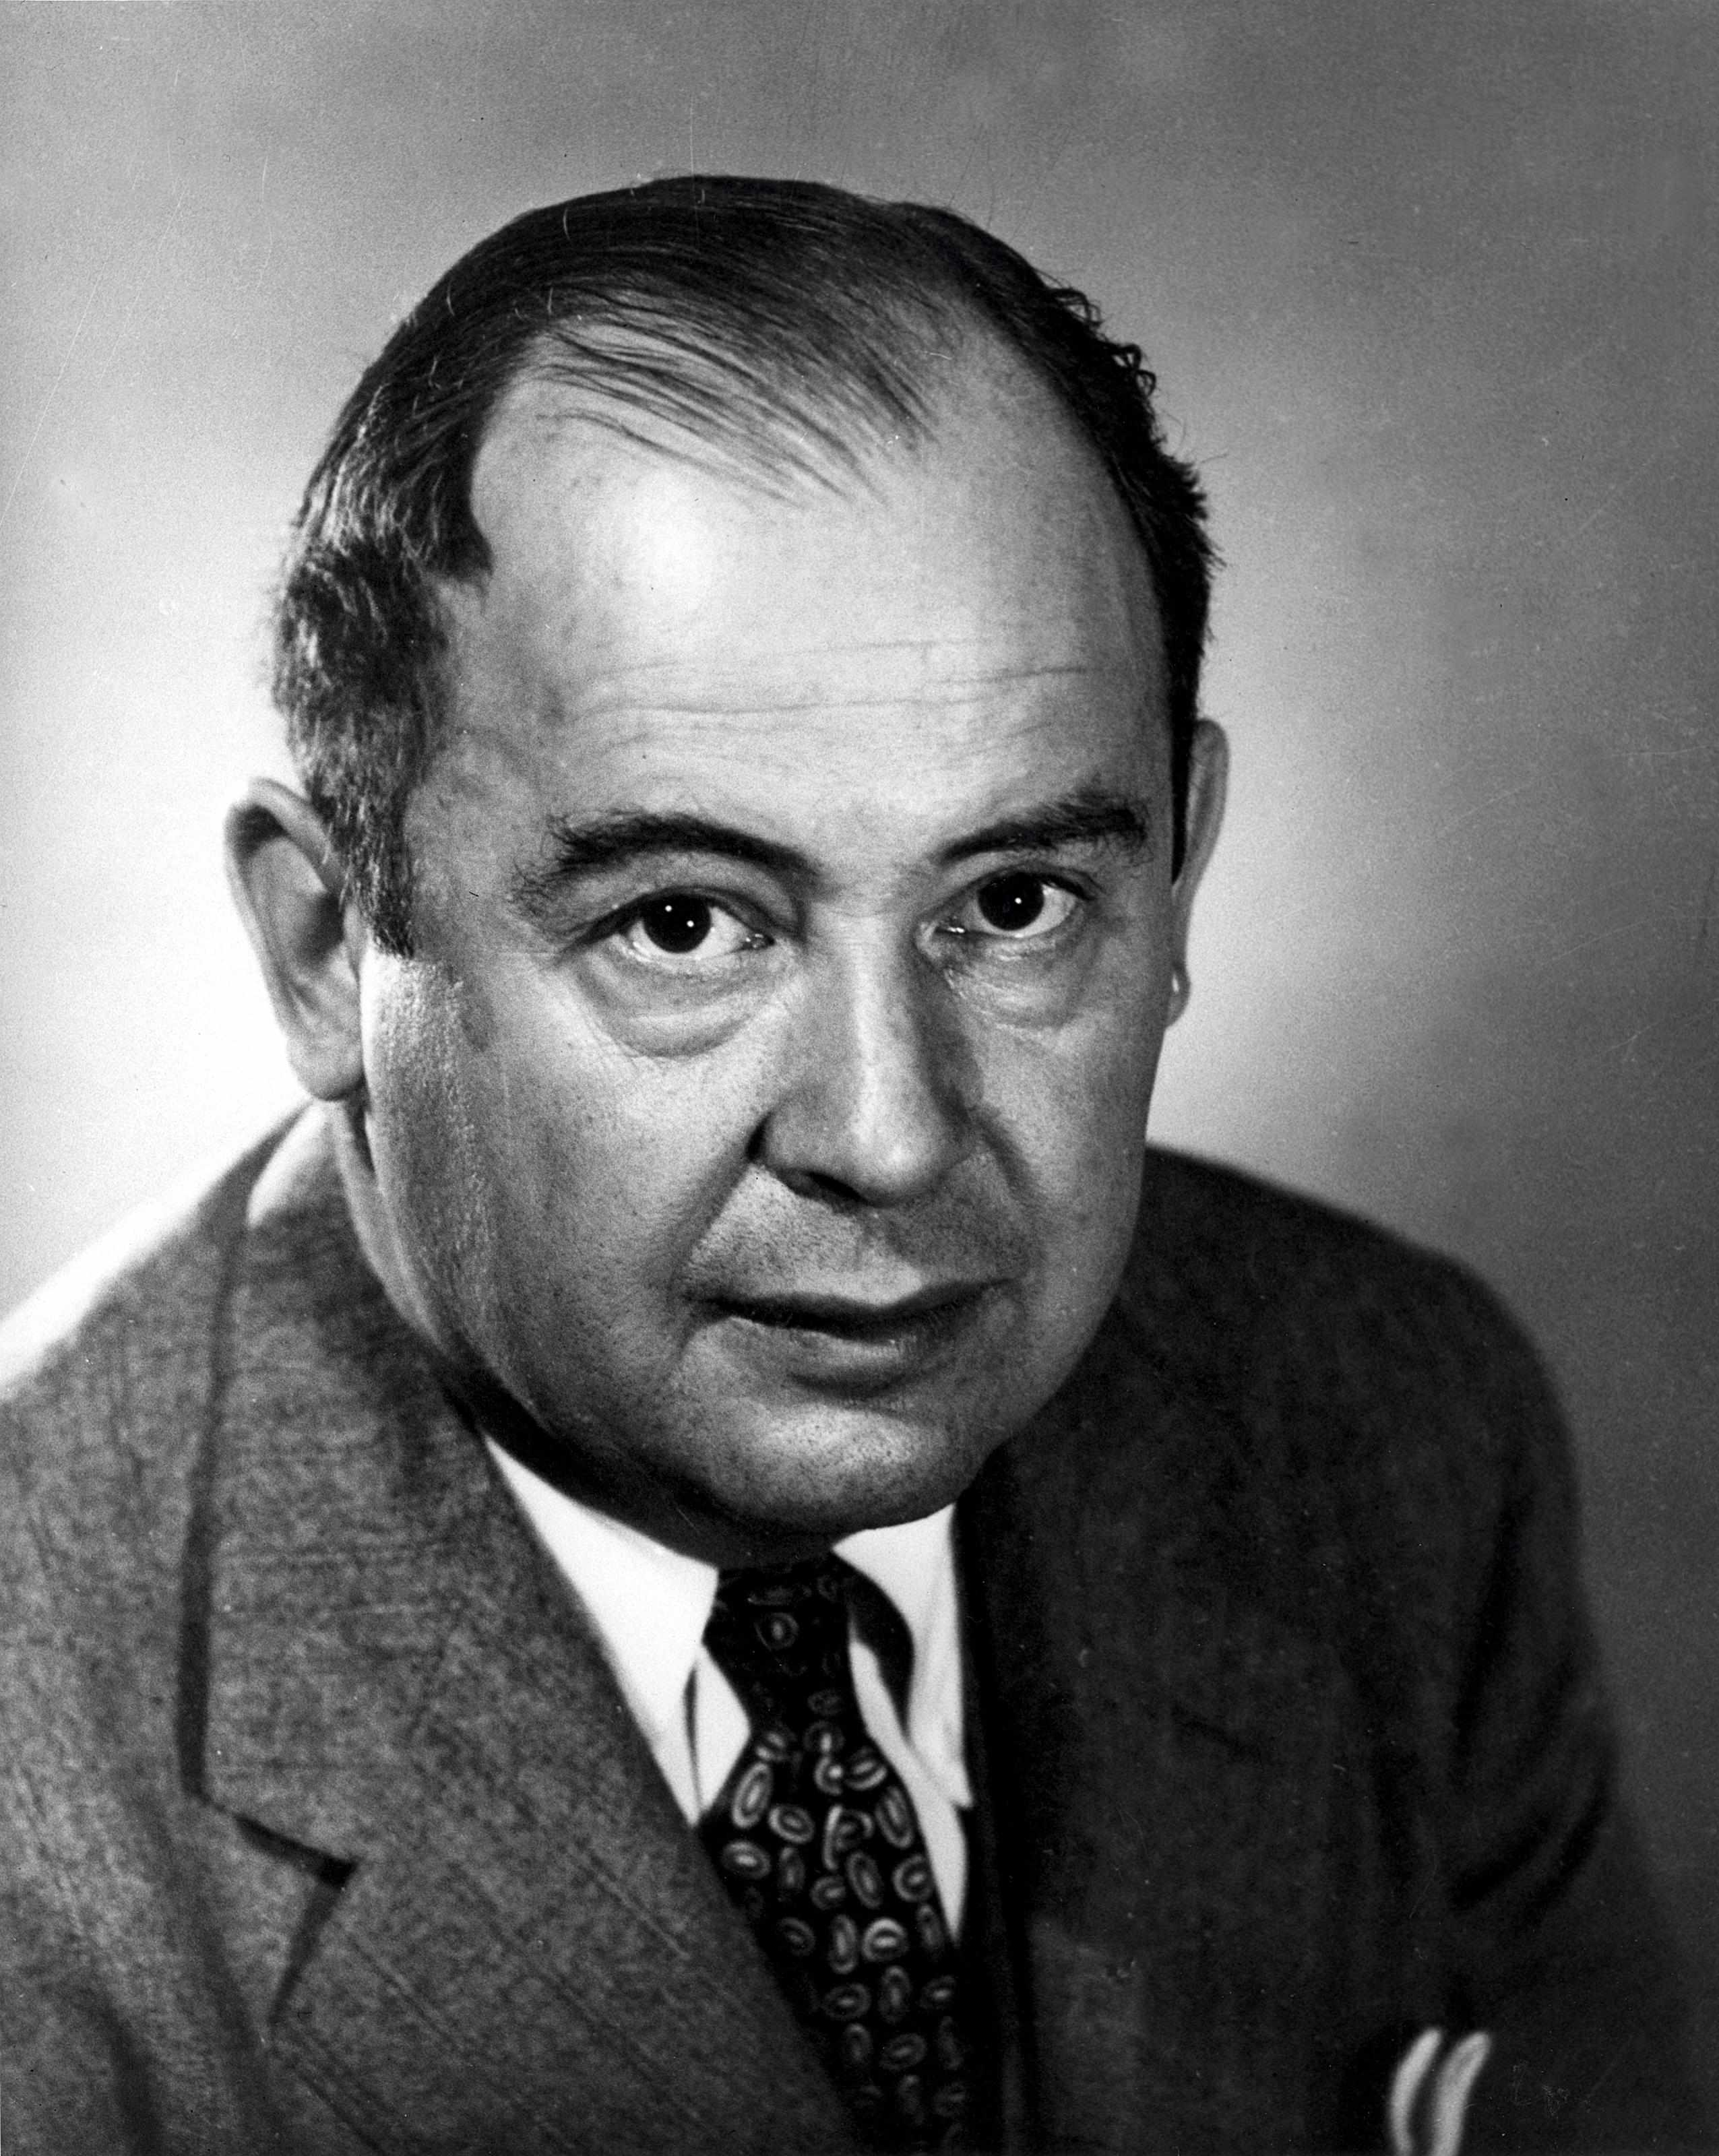
\includegraphics[scale = .03]{Images/JVN2.jpg}
      
    % \end{figure}


\end{frame}



\begin{frame}{Again some motivation}
  

    
    \begin{figure}
    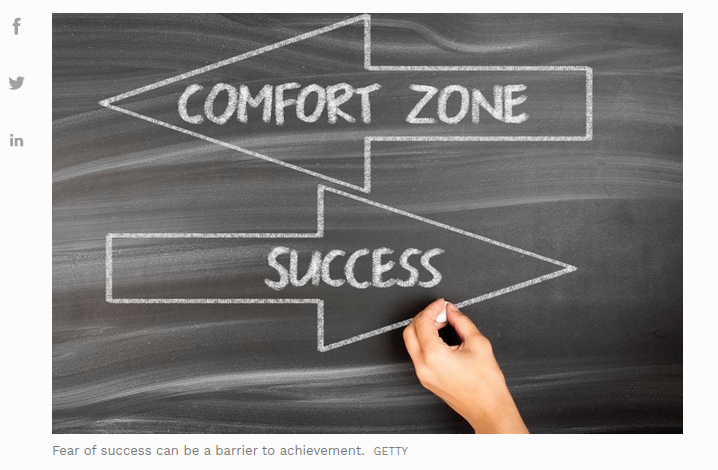
\includegraphics[scale = .3]{Images/fear_not.png}
    \caption{fear can be a barrier for success, so stop being scared and work hard, \url{https://www.forbes.com/sites/carolinecastrillon/2021/08/22/top-10-reasons-you-have-a-fear-of-success/?sh=54dde6da1c15}}
      
    \end{figure}


\end{frame}



\section[DataVariable]{Data and Variables}
\frame{\sectionpage}

\begin{frame}[allowframebreaks]{Data and Variables}
\begin{itemize}

\item Statistics starts from data, so let's consider the following hypothetical data set,

\begin{table}[H]
\begin{tabular}{l|c|c|c|c}
\hline
 & Gender & Monthly Income (tk) & ECO-101 Grade & \# Retakes\\
\hline
1. & Male & 3615 & B- & 3\\
\hline
2. & Female & 49755 & A & 2\\
\hline
3. & Male & 44758 & A & 1\\
\hline
4. & Female & 3879 & B & 0\\
\hline
5. & Male & 22579 & A+ & 2 \\
\hline
\end{tabular}
\end{table}


\item Here the columns are called \alert{variables} and the rows are called \alert{observations} or \alert{units}. We have $5$ observations and $4$ variables. Total number of observations is called \alert{sample size}, here the sample size is equal to $5$. 

\framebreak

\item We can classify the variables in different ways,

\bigskip

\textbf{\S. Whether we can group them or categorize them!}
\medskip
\begin{enumerate}
\item \alert{Categorical Variables}, also called \emph{Qualitative Variables}
\begin{itemize}
  \item  \textbf{Key Characteristic:} Values can be grouped 
  \item  \textbf{Examples:} Gender: Male / Female, Grade: Pass / Fail, Marital Status: Married / Unmarried
\end{itemize}
\medskip
\item \alert{Numeric Variables}, also called \emph{Quantitative Variables}
\begin{itemize}
  \item \textbf{Key Characteristic:} Values are numeric and represent how much or how many 
  \item  \textbf{Examples:} Monthly Income, Height, Weight, Exam Scores.
\end{itemize}
\medskip
\end{enumerate}


\bigskip

\textbf{\S.  Whether the values are discrete or continuous}
\medskip
\begin{enumerate}
\item \alert{Discrete Variables}
\begin{itemize}
  \item \textbf{Key Characteristic:} Only certain values (often integers) are possible, countable
  \item \textbf{Examples:}  Number of children - 0, 1, 2, 3, Number of times a student retakes a course 0,1,2,....
\end{itemize}
\medskip
\item \alert{Continuous Variables}
\begin{itemize}
  \item  \textbf{Key Characteristic:} Values can lie in a real interval or in set in $\mathbb{R}$ 
  \item \textbf{Examples:}  Income, Height, Weight, Time to finish a task.
\end{itemize}
\medskip
\end{enumerate}





\framebreak


\textbf{\S. How the values are compared or what is the scale of measurement}
\medskip
\begin{enumerate}
\item \alert{Nominal Scale}
\medskip
\begin{itemize}
  \item \emph{Categorical Variables} (e.g., gender, blood type) with \emph{NO intrinsic order}
  \item Example: “Gender - Male/Female,” “Fruits - Apple/Orange/Banana.”
  \item Important: You cannot say one category is “higher” or “greater” than another; only comment they are “different.”


\end{itemize}
\medskip
\item \alert{Ordinal Scale}
\medskip
\begin{itemize}
\item \emph{Categorical Variables} that can be \emph{ranked or ordered}, but differences between ranks may not be uniform.
\item Examples: Letter grades A/B/C, or Likert scale: Strongly Disagree < Disagree < Neutral < Agree < Strongly Agree)
\item Important: The difference between “Strongly Disagree” and “Disagree” may not be the same as the difference between “Neutral” and “Agree.”
\end{itemize}
\medskip
\item \alert{Interval Scale}
\medskip
\begin{itemize}
\item \emph{Numeric scale} where \emph{differences} are meaningful, but zero does not indicate “absence” of the quantity.
\item Typical For: Numeric variables (Quantitative) measured on a scale without a true zero.
\item Example: Temperature in Celsius or Fahrenheit ($0^{\circ}$C is not “no heat”).
\item Key Property: We can add or subtract values meaningfully, but a ratio (e.g., “twice as much”) is not valid.
\end{itemize}
\medskip
\item \alert{Ratio Scale}
\medskip
\begin{itemize}
  \item  This is a numeric scale that \emph{includes a true zero}, which means that both differences and ratios are meaningful (e.g., income, height, weight).
  \item Examples:   Income, height, weight, time to finish a task.
\end{itemize}


\end{enumerate}

\end{itemize}
\end{frame}



\begin{frame}[allowframebreaks]{Collection of data and different type of data}
  
\begin{itemize}

\item Now let's talk about \emph{how do we collect data}, roughly we can collect data using any of the following three methods,

\begin{itemize}

  \item by existing sources (e.g., administrative data sets)
  \item by conducting an observational study (e.g., by taking surveys)
  \item or by conducting an experiment.(e.g., giving training programs)


\end{itemize}


\item Depending upon \emph{space and time} we can also categorize the data in following three ways, 



  \begin{itemize}
  \item Cross-sectional data (data at same point in time, but for different units, e.g., household surveys at any fixed time)
  \item Time Series data (will have a time component, e.g., looking at GDP of Bangladesh for 10 consecutive years)
  \item It is also possible to have a combination of both, which we call Panel data.
  \end{itemize}


\end{itemize}
\end{frame}








%==================================================================================================



% \begin{}
  
% \end{}






\section{Population and Sample}
\frame{\sectionpage}


\begin{frame}[allowframebreaks]{Population Data Vs. Sample Data}
  
\begin{itemize}

  \item Before we go further, we need to talk about what do we mean by the word ``population''and  ``sample'' in Statistics? Consider the data set we saw before, someone may ask 

  \medskip
  \emph{``Why did we collect the \alert{data of 5 students} studying currently at EWU?''}
  \medskip
  
  \item One answer could be  

  \medskip
  \emph{``Maybe we are interested to get some idea about {\alert{all of the students}} studying currently at EWU.''} 
  \medskip

  \item In this case, we say the \alert{population} is the set of all current students at EWU. And the set of \alert{5 students} is a sample of that population. 



  \begin{varblock}{\Thm{Definition~} (Population and Sample) }
        The collection / set of \alert{all observations} in a particular study is called the population. A sample is a subset of the population. 
  \end{varblock}


    \framebreak

  \item Usually collecting population data is very time consuming and often impossible, for example ???

  \item So we collect \emph{a sample} from the population.

  \item Note that a sample is supposed to be a good representative of the whole population.

  \item If the sample is not a good representative, then we say we have a \alert{biased sample}.

  \item Biased sample is bad, why?... because any conclusion from a biased sample might lead to incorrect conclusion regarding the population (can you think about an example?)


  \framebreak

  \item One way to get a good sample is - \alert{Simple Random Sampling!} (details on board)

  \item What if the population is infinite ??? Is it even possible in reality ???

  \item
  One of the major tasks of statistical analysis is, using a sample to make some conclusions regarding the population. This process is called \alert{Statistical Inference}, or we call this - \alert{Inferential Statistics}.

  \item In this course, we will not talk about Inferential Statistics. But in ECO 204, you will learn some techniques related to Inferential Statistics. 

  \item However let's do an example on board! (Population Mean Vs. Sample Mean).

  \item Here we are making inference about Population Mean using Sample Data!



\end{itemize}

\end{frame}








\section{Descriptive Statistics - Tabular and Graphical Methods}
\frame{\sectionpage}


\begin{frame}[allowframebreaks]{Descriptive Statistics}
\begin{itemize}

   \item Now we will start with descriptive statistics, which is the first major topic of this course. Recall in \emph{Inferential Statistics}, we try to use the sample data to \alert{comment / infer} about the population.

   \item \emph{Descriptive Statistics} is simpler, in descriptive statistics we don't make any conclusion about population, the only thing we have is data, so with different procedures we will comment on data, that's it.  Essentially the idea of a descriptive statistical analysis is  to \alert{summarize the data} so that the key information \alert{in the data} are clear, whether we do it \alert{visually or numerically}


  \item There are two ways we can do descriptive statistical analysis (or descriptive statistics!)

  \begin{itemize}
    \fontsize{8}{12}\selectfont
     \item Tabular and Graphical Methods
     \item Numerical Methods
   \end{itemize} 

 \framebreak

\normalsize{
\item We will cover following Tabular and Graphical methods! Tabular and Graphical Methods are often discussed together since most of the times, first we have some tables and then we convert the table into some graphs. 

\begin{itemize}
  \normalsize
  \medskip
  \item \textbf{For Single Variable:}
  \medskip
  \begin{enumerate}
    \normalsize
      \item \alert{Frequency Distribution Table (Tabular)} and \alert{Bar Chart and Pie Chart (Graphical)}\\
            (All are applicable only for \emph{categorical} variables.)
      \item[]
      \item \alert{Grouped Frequency Distribution Table (Tabular)} and \alert{Histogram (Graphical)}\\
            (Only applicable for \emph{numeric} variables.)
  \end{enumerate}
  

  \medskip
  \item A side note: The Frequency Distribution (or Relative Frequency or Percent Frequency Distribution) is a \emph{tabular method}. There is no graphical element here; rather, it provides the table used to create bar charts and pie charts, which are graphical methods.
  
\framebreak

  \medskip
  \item \textbf{For Two Variables:}
  \medskip
  \begin{enumerate}
    \normalsize
      \item \alert{Cross-tabulation or Contingency Table or Joint Frequency Distribution (Tabular)} and \alert{Side-by-Side Bar Chart or Stacked Bar Chart (Graphical)}\\
            (Applicable for \emph{two categorical} variables.)
      \item[]
      \item \alert{Bivariate Frequency Distribution Table (Tabular)} and \alert{Joint Histogram (3D Histogram) (Graphical)}\\
            (Applicable for \emph{two numeric} variables.)
      \item[]
      \item \alert{Scatter Plot (Graphical)}\\
            (Applicable for \emph{two numeric} variables to understand association.)
  \end{enumerate}

\end{itemize}
}



%   \begin{itemize}

% \medskip
%   \item[] \textbf{For Single Variable:}

%   \item[] 1. \alert{Frequency Distribution Table (Tabular)} and  \alert{Bar Chart and Pie Chart (Both Graphical)} (all are applicable only for \emph{Categorical} variables)

%   \item[] 2. \alert{Grouped Frequency Distribution Table (Tabular)}, and \alert{Histogram (Graphical)}  (only applicable for \emph{Numeric} variables)

%   \item[]

%   \item[] A side note: We will see that Frequency Distribution (or Relative Frequency or Percent Frequency Distribution) is a \emph{tabular method}, there is no graphical thing here, but this gives the table which we use to create Bar chart and Pie chart which are graphical methods.

%   \item[]
%   \item[] \textbf{For Two Variables:}

%   \item[] 1. \alert{Cross-tabulation or Contingency Table (Tabular) or Joint Frequency distribution (Tabular)} and  \alert{Side by Side Bar Chart or Stacked Bar Chart (Graphical)} (applicable for \emph{two categorical variables

%   \item[] 2. \alert{Joint Grouped Frequency Distribution Table (Tabular)} and \alert{Joint Histogram (3D histogram)} (applicable for \emph{two numeric variables})

%   \item[] 3. \alert{Scatter Plot} (this is for \emph{two numeric variables but understanding association})


% \end{itemize}

\medskip

\item The cross-tabulation can also be applied for a combination of \emph{categorical and numeric variables}, we will see some examples.



\end{itemize}
\end{frame}



% \subsection{Bar Chart}

\subsection{Single Variable Methods (Qualitative): Frequency Distribution, Bar Charts and Pie Charts}
\frame{\subsectionpage}



\begin{frame}[allowframebreaks]{Frequency Distribution and Bar Charts}

\begin{itemize}
\item We will start with \emph{frequency distribution}, a tabular method for describing categorical data.

\medskip
\begin{varblock}{\Thm{Definition~} (Frequency and Frequency Distribution)}
  \begin{itemize}
    \normalsize
    \item \textbf{Frequency:} The number of observations in a given category.
    \item \textbf{Frequency Distribution:} A \alert{frequency distribution} is a \emph{tabular summary} that displays the frequency (i.e., the number of observations) for each category.
  \end{itemize}
\end{varblock}

\medskip
We will also look at two related concepts 

\medskip
\begin{itemize}
 \item \alert{Relative Frequency Distribution}: This shows the \emph{fraction or proportion} of observations for each category.
 \medskip 
 \item \alert{Percent Frequency Distribution}: Shows the \emph{percentage} of observations for each category. 
\end{itemize}
  
  \medskip

Let’s consider an example. Suppose we have sales data from a supershop that shows which soft drink was sold in the last 50 transactions. Here is how the data looks:

 \framebreak 

  \begin{figure}[H]
  \center
    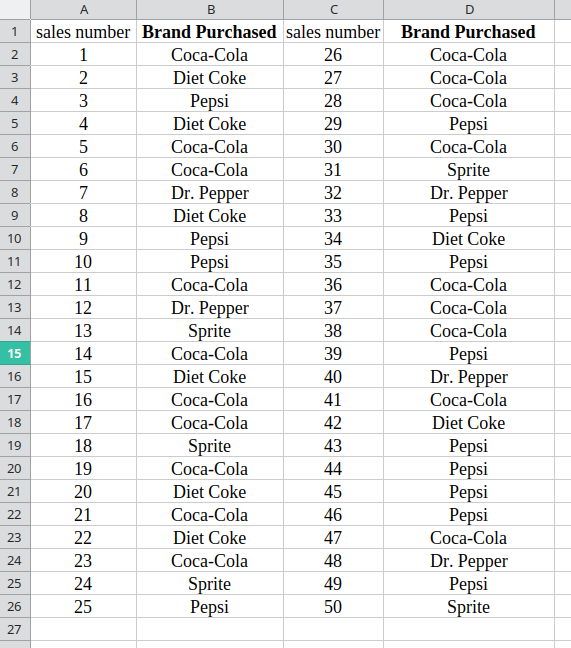
\includegraphics[scale = .4]{Images/Sales_data.png}
  \end{figure}

  \framebreak

  \item The frequency distribution, percent frequency distribution and relative frequency distribution in this case is,

\medskip

    \begin{table}

    \begin{tabular}{c|c|c|c}
      \hline Brand & Frequency & Relative Frequency & Percent Frequency \\
      \hline Coca-Cola & 19 & 0.38 & 38 \\
      \hline Diet Coke & 8 & 0.16 & 16 \\
      \hline Dr. Pepper & 5 & 0.1 & 10 \\
      \hline Pepsi & 13 & 0.26 & 26 \\
      \hline Sprite & 5 & 0.1 & 10 \\
      \hline Grand Total & 50 & 1 & 100 \\
      \hline
\end{tabular}
  \end{table}



\framebreak

\item[] \textbf{An important side note:} 

\medskip

Notice that the term \emph{distribution} is used here because the relative and percent frequency distributions actually represent the \alert{probability distribution} of each category. In other words, they show how the overall probability of sales is allocated among the different categories.

\medskip

Roughly probability gives us a measure of \emph{likelihood / chance / percentage of happening certain events}, for example if someone asks, 

\medskip
\begin{center}
  \emph{what is the probability that the next sale will be Coca-Cola?}
\end{center}

\mnedskip


Based on the data, we might conclude that,


\mnedskip

\begin{center}
\alert{Well, we have actually 38\% chance that the next sales will be Coca-Cola}
\end{center}
\mnedskip


We’ll explore probability in more depth in the next chapter, but for now, the key takeaway is that percent frequency distributions provide a practical approximation of the probability distribution of sales of all categories. This understanding will be very important to understand probability distribution of a random variable later... so keep this in mind. 

% \item Now let's see how to do this in Excel

%   \framebreak


%   \item We need to do two tasks, \emph{1. Enter / Access Data} and \emph{2. Apply Tools that MS-Excel gives}.

%   \item \emph{1. Enter / Access Data:} We already have the data, so no need to enter, just open the file \texttt{SoftDrink.xlsx}. The data are in cells \texttt{A2:A51} and a \emph{label} is in cell \texttt{A1}.

%   \item \emph{2. Apply Tools:} Do following steps

%   \begin{itemize}
%     \item[] \textbf{Step 1} Select any cell in the data set (from cells \texttt{A1:A51})
%     \item[] \textbf{Step 2} Click the Insert tab on the ribbon and click \alert{Recommended PivotTables}\footnote{What is a PivotTable?, we will talk about this later!}, you should already see a preview of the frequency distribution table.
%     \item[] \textbf{Step 4} Click OK; the frequency distribution will appear in a new worksheet
%     \item[] \textbf{Step 5} Copy the entire table and \alert{paste values} in a new range, maybe below (this will remove the formulas inside the table), and in this way we can also create other numbers

%     \item \textbf{Step 6} Rename the columns, first column ``Brand'' and second column ``Frequcny''

%     \item[]\textbf{Step 7} Now create two additional column ``Relative Frequency'' and ``Percent Frequency''

%     \item[]\textbf{Step 8} To create ``Relative Frequency'' divide the cell value with total (careful you need to use \$ in Excel)

%     \item \textbf{Step 8} To create ``Percent Frequency'' is just multiplying by 100


\framebreak

\vspace*{-1cm}
\item Now the bar chart is, 

\begin{figure}[H]
  \caption{Bar Chart of Soft Drink Purchases}
  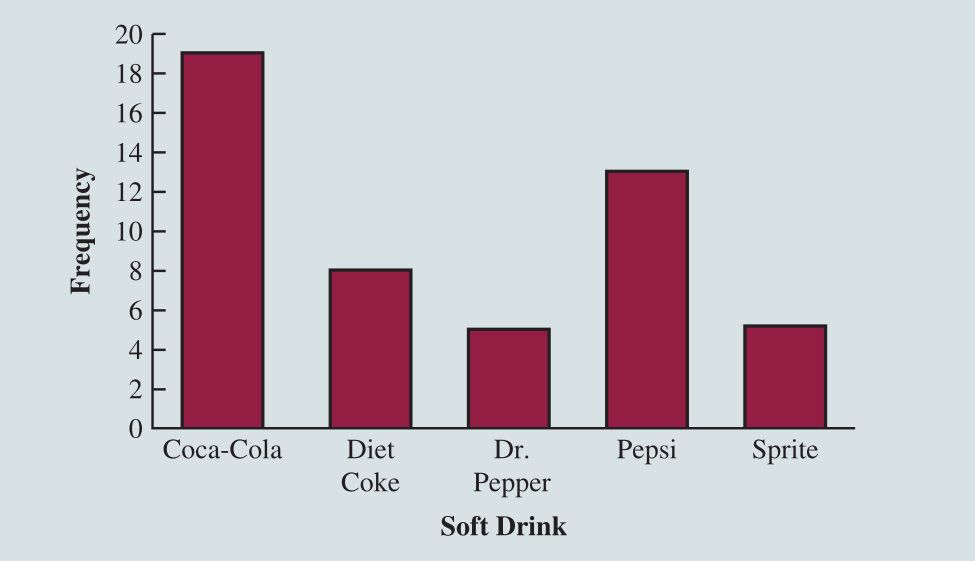
\includegraphics[scale = .2]{Images/SoftDrink_BarChart.png}
\end{figure}


\item It is possible to sort the table in ascending order to create a more visually appealing bar chart in Excel. What does the bar chart convey, and how would you interpret it

\item Ans: The bar chart shows that the highest sales occur for Coca-Cola and Pepsi, indicating that consumer preferences in that region favor these brands. In contrast, the lowest sales are recorded for Dr. Pepper and Sprite, suggesting these brands are less popular among consumers.







\end{itemize}


  
\end{frame}


\begin{frame}[allowframebreaks]{Pie Chart}
\begin{itemize}

\item From the frequency distribution table, we can also construct a pie chart as well. Here is how Pie Chart looks like (we will do this in Excel, note the message is same!)

\begin{figure}
  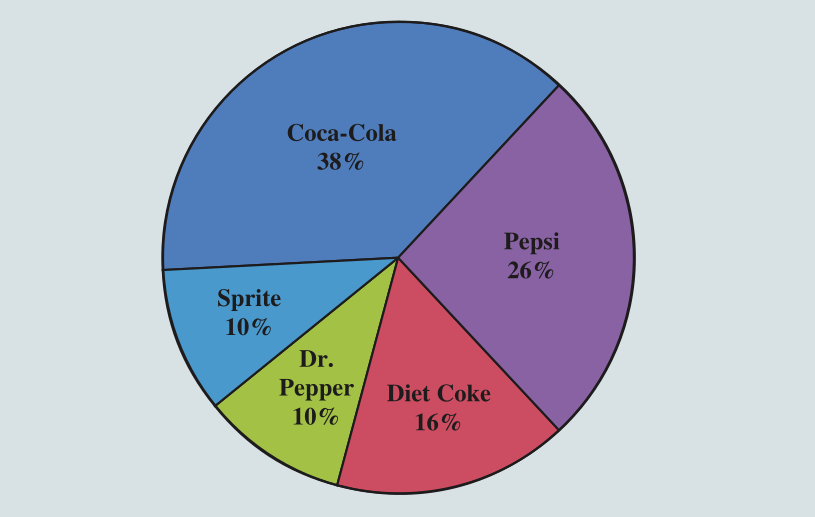
\includegraphics[scale = .3]{Images/SoftDrink_PieChart.png}
\end{figure}




\end{itemize}
\end{frame}


\subsection{Single Variable Methods (Quantitative): Histogram}
\frame{\subsectionpage}

\begin{frame}[allowframebreaks]{Histogram}
\begin{itemize}

\item  If we are looking for a summary measure of a numeric variable, then it is not a good idea to use bar chart / pie chart directly, Why? because there are just too many different values in the data set tp treat them as categories.  So we need a \emph{new} graphical method to understand the numeric variables, this is where \emph{histogram} comes.Consider the following data of an audit firm which shows the number of days required to audit different companies. Let's create a histogram from this data.

% \framebreak

\begin{figure}
  \caption{Data From \citet*{anderson_statistics_2020}'s book}
  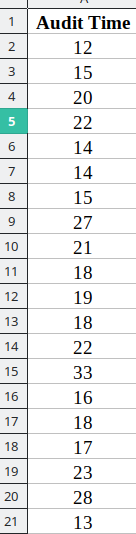
\includegraphics[scale = .3]{Images/Audit_Data.png}
\end{figure}

\item  To create a histogram, we first craete \emph{bins} or \emph{classes}. In this example, we create 5 bins: $10-14$, $15-19$, $20-24$, $25-29$, and $30-34$. We then count how many data points fall into each bin, which gives us a frequency distribution similar to what we saw before—but now for a numeric variable. This is what we call \emph{grouped frequency distribution},


    \begin{table}


    \begin{tabular}{c|c}
      \hline Audit Time (Days) & Frequency   \\
      \hline 10 -14 & 4 \\
      \hline 15 - 19 & 8  \\
      \hline 20 - 24 & 5  \\
      \hline 25 - 29 & 2  \\
      \hline 30 - 34 & 1  \\
      \hline Total & 20 \\
      \hline
\end{tabular}
  \end{table}


We can also calculate the \emph{relative frequency} and \emph{percent frequency} for each bin, as well as the \alert{cumulative percent frequency}, which shows the running total of percentages as we include more data.




    \begin{table}


    \begin{tabular}{c|c|c|c|c}
      \hline Audit Time (Days) & Frequency & Relative Freq & Percent Freq & Cum Percent Freq  \\
      \hline 10 -14 & 4 & .20 & 20 & 20  \\
      \hline 15 - 19 & 8 & .40 & 40 & 60 \\
      \hline 20 - 24 & 5 & .25 & 25 & 85 \\
      \hline 25 - 29 & 2 & .10 & 10 & 95 \\
      \hline 30 - 34 & 1 & .05 & 5 & 100 \\
      \hline Total & 20 \\
      \hline
\end{tabular}
  \end{table}


\farmebreak

\item Next, we convert the first table into a graph like a bar chart, which is known as a \emph{histogram}. Here is the resulting histogram:

\medskip
\begin{figure}[H]
  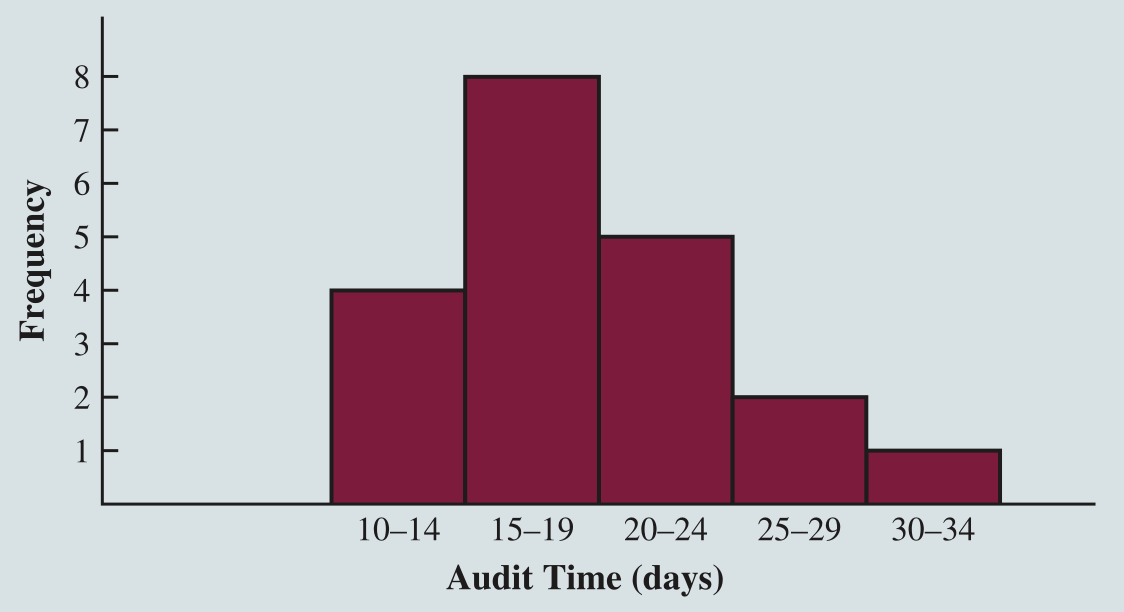
\includegraphics[scale = .2]{Images/Audit_Histogram.png}
\end{figure}

\framebreak


\item You might notice that a histogram looks similar to a bar chart. While this is true, there is a fundamental difference: 

\medskip
\begin{center}
  \alert{bar charts display categorical variables, whereas histograms display quantitative variables}
\end{center}

\medskip


\item The visual representation is similar, but the nature of the data is quite different, also unlike the bar chart, the bars here have no space between them, this is because we have a continuous numeric data, not a discrete / categorical one.

\item Can you interpret the histogram? It appears that the majority of the data falls within the $15-19$ range. This suggests that most audits are completed within 15 to 19 days.


\framebreak

\item In the last example, we first picked the number of bins $k = 5$, then we calculated the bin-width $h$ using the formula (here we let $k$ be the number of bins then, $h$ be the bin-width)


\begin{align*}
  h \approx \frac{\text{maximum} - \text{minimum}}{k} = \frac{35 - 10}{5} = 5
\end{align*}

\item After that, we get the bins, $10-14$, $15-19$, $20-24$, $25-29$, and $30-34$.

\item Note $33$ and $12$ is the max and min but we picked $35$ and $10$ just to get a round figure when we divide the difference by $5$.

\framebreak

\item Two million dollar questions are, 1) Why did we choose $5$ as the number of bins, and 2) What happens if we increase the number of bins? 

\item Let's answer the second question first, if increase the number of bins then each bin cover a smaller range, so yes we might see more details about the data’s distribution. 


\item However, if we use too many bins, the histogram might become too "noisy" with many bins having very few observations, making it harder to see overall patterns in the data. 

\item Conversely, too few bins can oversimplify the data, hiding important patterns also. The key is to find a balance that provides meaningful insight without excessive detail or oversimplification. 


\framebreak


\item Now we answer the first one, there different techniques to select number of bins or bin-width, but there is no single technique that works best always. 

\item Here are two common techniques,


\medskip
\begin{itemize}
  \item 1. Square Root Rule, which says

\begin{align*}
  k=\sqrt{n}
\end{align*}


where $n$ is the sample size. This rule is straightforward and often used for a quick estimate.

\medskip

\item 2. Freedman-Diaconis Rule, which says

Instead of directly giving the number of bins, it provides a bin width:

$$
h=2 \times \frac{\mathrm{IQR}}{n^{1 / 3}}
$$


where $IQR$ means inter-quartile range (we will see how to calculate this in the next section), then the number of bins can be calculated as:

$$
k=\frac{\text { Range }}{h}
$$


This rule is useful when you want to balance the bin width against the variability in the data.
\end{itemize}







% \item Here is how to do it Excel 

% \begin{itemize}
%   \item \textbf{Step 1.} Select any cell in the data set (cells A1:A21)
%   \item \textbf{Step 2.} Click the Insert tab on the Ribbon
%   \item \textbf{Step 3.} In the Tables group click PivotTable
%   \item \textbf{Step 4.} When the Create Pivot Table dialog box appears:
%   Click OK; a PivotTable and PivotTable Fields task pane will appear in a new worksheet
%   \item \textbf{Step 5.} In the PivotTable Fields task pane:
%   Drag Audit Time to the ROWS area
%   Drag Audit Time to the VALUES area
%   \item \textbf{Step 6.} Click on Sum of Audit Time in the VALUES area
%   \item \textbf{Step 7.} Select Value Field Settings... from the list of options that appears
%   \item \textbf{Step 8.} When the Value Field Settings dialog box appears:
%   Under Summarize value field by, choose Count Click OK

%   \item \textbf{Step 9.} Right-click cell A4 in the PivotTable or any other cell containing an audit time
%   \item \textbf{Step 10.} Choose Group from the list of options that appears

%   \item \textbf{Step 11}. When the Grouping dialog box appears, Enter 10 in the Starting, Enter 34 in the Ending, and Enter 5 in and Click OK
% \end{itemize}






\end{itemize}
\end{frame}


\subsection{Two Variable Methods (Qualitative): Cross Tabulation, Two Variate Bar Charts}
\frame{\subsectionpage}


\begin{frame}[allowframebreaks]{Cross Tabulation}

\begin{itemize}

  \item So far we only talked about graphical methods using a single variable, now we will consider methods using two variables together.

  \item The idea of cross tabulation is very similar to frequency distribution, but here we have two variables. 

  \item We can construct cross tabulation in three ways,

  \begin{itemize}
    \item Both variables can be categorical, in this case this is often known as \emph{contingency table}.

    \item One variable can be categorical and the other can quantitative.

    \item Both variables can be quantitative.
  \end{itemize}


\item Let's see some examples (we will see how to create this tables in Microsoft Excel in the lab class.)


\end{itemize}
  
\end{frame}



\begin{frame}[allowframebreaks]{Cross Tabulation}{Both Categorical}

\begin{itemize}
  \item Consider following data (Right-H means Right Handed, and Left-H means Left-Handed)

\begin{table}
  \begin{tabular}{cccccc} 
Observation & \emph{Handed} & \alert{Male/Female} & Observation & \emph{Handed} & \alert{Male/Female} \\
1. & Right-H & Male & 16.& Left-H & Female \\
2. & Left-H & Male & 17.& Left-H & Male \\
3. & Left-H & Male & 18.& Left-H & Male \\
4. & Right-H & Female & 19.& Right-H & Male \\
5. & Left-H & Male & 20.& Left-H & Male \\
6. & Right-H & Female & 21.& Right-H & Female \\
7. & Left-H & Male & 22.& Left-H & Male \\
8. & Left-H & Female & 23.& Left-H & Female \\
9. & Right-H & Male & 24.& Right-H & Male \\
10. & Left-H & Male & 25.& Left-H & Male \\
11. & Right-H & Male & 26.& Left-H & Female \\
12. & Left-H & Male & 27.& Left-H & Female \\
13. & Left-H & Female & 28.& Right-H & Male \\
14. & Left-H & Female & 29.& Left-H & Male \\
15. & Left-H & Female & 30. & Left-H & Female 
\end{tabular}
\end{table}


\item With this table we can construct following crosstabulation or contingency table,

\begin{table}
  \begin{tabular}{|l|r|r |r|}
\hline  & \alert{Female}  & \alert{Male} & Total Result   \\
\hline \emph{Left-H} & 9 & 12 & 21 \\
\emph{Right-H} & 3 & 6 & 9 \\
\hline Total Result & 12 & 18 & 30 \\
\hline
\end{tabular}
\end{table}

\item Here each variable in the data set has 2 categories, so in total we have $4$ categories, 

\begin{itemize}
  \item Right Handed Male (count - 6)
  \item Right Handed Female (count - 3)
  \item Left Handed Male (count - 12)
  \item Left Handed Female (count - 9)
\end{itemize}

\item We can also calculate the percentages? How ?

\item We can also calculate Row total or Row Percentages, this means

\begin{itemize}
  \item Total Number of Left Handed people, or Total Percentage of Left Handed people.
  \item Total Number of Right Handed people, or Total Percentage of Right Handed people.
\end{itemize}

\item We can also calculate Column total or Column Percentages, this means

\begin{itemize}
  \item Total Number of Male, or Total Percentage of Male.
  \item Total Number of Female, or Total Percentage of Female.
\end{itemize}

  
\item We will also see how to calculate these numbers using MS-Excel in our lab class.

\end{itemize}
\end{frame}





\begin{frame}[allowframebreaks]{Cross Tabulation}{One Categorical and One Quantitative}

\begin{itemize}

\item It is also possible to construct a crosstabulation when one variable is categorical and the other is quantitative. 

\item For example, consider following data which is collected from $300$ restaurants (only partially shown, the data is available in the file \texttt{Restaurant.xlsx} file in chapter 2)

\begin{table}
\begin{tabular}{clc} 
Restaurant & Quality Rating & Meal Price (\$) \\
1. & Good & 18 \\
2. & Very Good & 22 \\
3. & Good & 28 \\
4. & Excellent & 38 \\
5. & Very Good & 33 \\
6. & Good & 28 \\
7. & Very Good & 19 \\
8. & Very Good & 11 \\
9. & Very Good & 23 \\
10. & Good & 13 \\
\vdots & \vdots & \vdots \\
\vdots & \vdots & \vdots \\
300. & Very Good & 31 \\
 \end{tabular}
\end{table}

\item Here we have two kinds of variables, \texttt{Quality Rating} is a categorical variable and \texttt{Meal Price} is a quantitative variable. 

\framebreak

\item It is also possible to construct cross tabulation using this data, here is a crosstabulation that we can make using this data.

\begin{table}
  \begin{tabular}{l|cccc|c}
\multicolumn{5}{c}{ Meal Price } \\
Quality Rating & $\mathbf{\$ 1 0 - 1 9}$ & $\mathbf{\$ 2 0 - 2 9}$ & $\mathbf{\$ 3 0 - 3 9}$ & $\mathbf{\$ 4 0 - 4 9}$ & Total \\
\hline Good & 42 & 40 & 2 & 0 & 84 \\
Very Good & 34 & 64 & 46 & 6 & 150 \\
Excellent & 2 & 14 & 28 & 22 & 66 \\
\hline \multicolumn{1}{c|}{ Total } & 78 & 118 & 76 & 28 & 300
\end{tabular}
\end{table}

\item Notice the columns are like histogram categories, where a qunatitative variable is categorized in different categories, and then we calculated the frequency of each combination of categories.


\item In the lab class we will try to do this using MS-Excel, but now you know how it looks like.

\item What is the interpretation of $42$?

\item Similarly we can construct crosstabulation for two quantitative variables as well.


\end{itemize}

\end{frame}  

\begin{frame}[allowframebreaks]{Side by side bar chart or stcaked bar chart}
  
\begin{itemize}
  \item Once we have the crosstabulation we can also plot the side by side bar chart oor stacked bar chart


  \begin{figure}
  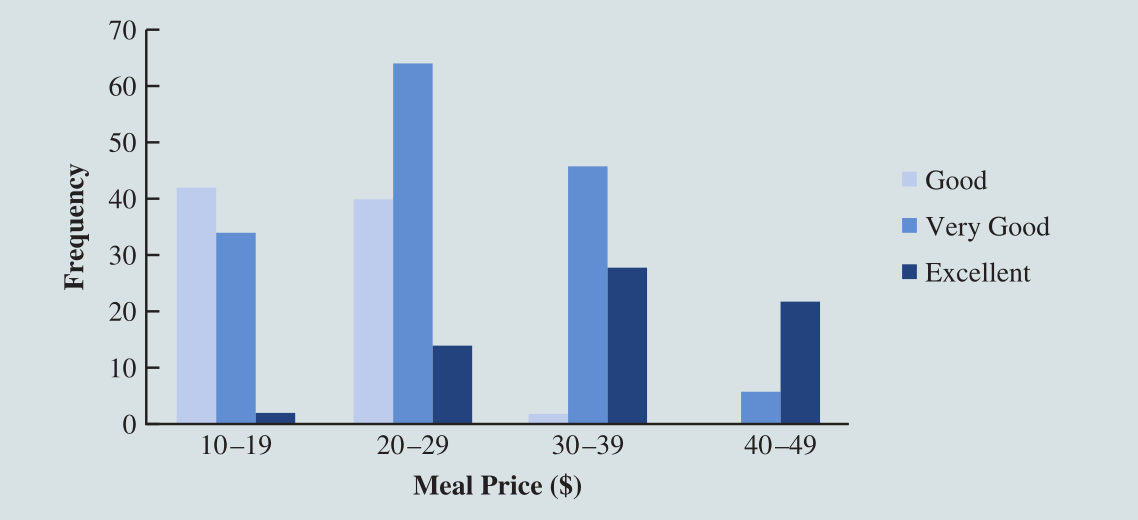
\includegraphics[scale = .203]{Images/barchart_sidebyside.png}  
  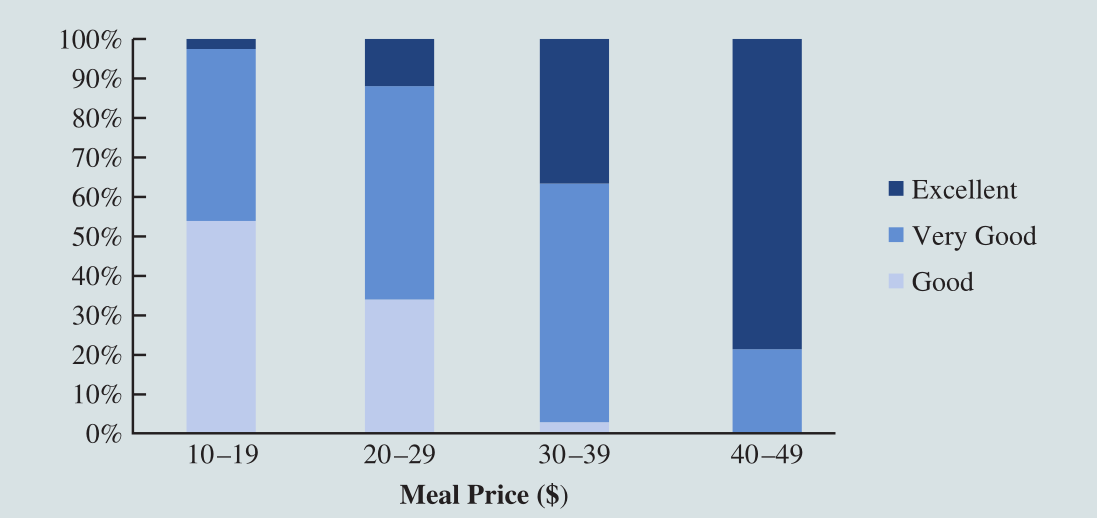
\includegraphics[scale = .21]{Images/barchart_stacked.png}
  \caption{The top one is the side by side bar chart and the bottom one is called stacked bar chart}
  \end{figure}

  \item Note that these are also bar charts, but the important thing is these type of bar charts are for two variables.

\end{itemize}
\end{frame}

\section{Descriptive Statistics - Numerical Measures}
\frame{\sectionpage}



\subsection{1. Measures of Location - Mean, Median and Percentile}
\frame{\subsectionpage}

\begin{frame}{Sample Mean (Arithmetic Mean)}


\begin{itemize}


\item In the last section we discussed some \alert{tabular} and \alert{graphical methods} to summarize a data, now we will see some \emph{numerical measures} that provide more ways for summarizing a data. It is possible to have numerical summary measures for a single variable or for more variables, first let's focus on one variable.

\item We will start with a measure of \alert{central location} of any data. The most common measure of the central location is the \emph{sample average} or \emph{sample mean}. Think about a variable \textit{height} and assume we have some kind of height data for $10$ students, then the following is a sample.

\begin{table}[H]
\begin{align*}
    \begin{array}{|r|r|}
    \hline
\text { student } & \text { heights } \\
\hline 1 & 5.5 \\
\hline 2 & 4.8 \\
\hline 3 & 5.2 \\
\hline 4 & 4.5 \\
\hline 5 & 6 \\
\hline 6 & 5.9 \\
\hline 7 & 6.2 \\
\hline 8 & 5.3 \\
\hline 9 & 6 \\
\hline 10 & 5 \\
\hline
\end{array}
\end{align*}

\end{table}

\end{itemize}





\end{frame}


% \begin{frame}[fragile]{NAME}

% \begin{lstlisting}[language=R]
% print("hello")
% \end{lstlisting}
    
% \end{frame}


\begin{frame}[allowframebreaks]{Sample Mean (Arithmetic Mean)}


\begin{itemize}


\item Usually we will write $x_1, x_2, \ldots, x_n$ rather than numbers $5.5, 4.8, 5.2, \ldots, 5$. This is just to generalize the writings. Now the sample mean can be calculated as 

$$
\bar{x}=\frac{1}{n}\sum_{i = 1}^{n} x_i = \frac{1}{10}(5.5 + 4.8 + \ldots + 5) = 5.44
$$



\item You can calculate this by hand, or using calculator, or using \texttt{MS-Excel}!

\item So the \emph{sample mean} (another name is \emph{arithmetic mean}) is simply the average value, it gives an idea of the center location of the data.

\framebreak

\item[] \textbf{Issues with sample mean}
\medskip
\item There is one issue with the Mean, that is, it changes drastically with \alert{extreme values}, for example, if we replace the $10$th observation with $20$ (which is unrealistic, but just to give you an example), then the sample mean would be $6.94$. So what happens is, if we change one value, the sample mean changes a lot, we say sample mean is not a \emph{robust} measure!

\item Later we will see another measure of central location which is \emph{sample median}, which is more robust than sample mean!

\end{itemize}





\end{frame}


\begin{frame}[allowframebreaks]{Weighted Mean}

\begin{itemize}

\item In the formulas for the sample mean each $x_i$ is given equal importance or weight. For instance, the formula for the sample mean can be written as follows:

\begin{align*}
  \bar{x}=\frac{1}{n}\sum_{i = 1}^{n} x_i=\frac{1}{n}\left(x_1+x_2+\cdots+x_n\right)=\frac{1}{n}\left(x_1\right)+\frac{1}{n}\left(x_2\right)+\cdots+\frac{1}{n}\left(x_n\right)
\end{align*}



\item This shows that each observation in the sample is given a weight of $1 / n$. 

\item Although this is very common, but sometimes we might give different weights to different observations  depending upon its relative importance. A mean computed in this manner is referred to as a \emph{weighted mean}. The formula is following


\begin{align}\label{eq:weighted_mean1}
  \bar{x}_n=\sum_{i = 1}^{n} w_i x_i
\end{align}

\item Note that, the weights have to be summed to $1$. Here is an example, 

\framebreak
  
\item Suppose we have following data of different costs of purchase, but notice each time the cost changes with number of pounds


\begin{align*}
\begin{array}{r|r|r}
\text{Number of Purchase} & \text{Cost per pound} & \text{Number of Pounds} \\ \hline
1 & 3.00 & 1200 \\
2 & 3.40 & 500 \\
3 & 2.80 & 2750 \\
4 & 2.90 & 1000 \\
5 & 3.25 & 800
\end{array}
\end{align*}

\item Now simple arithmetic mean would be average of all costs. If you calculate this you will get,

\begin{align*}
   \text { Arithmetic Mean }=\frac{3.00+3.40+2.80+2.90+3.25}{5}=\frac{15.35}{5}=3.07 \text {. }
 \end{align*} 



\item Now we will see the weighted average of costs will be different. We do here weighted average because the costs are not always same for every pound since amount of purchase is different. For the weighted average, first we calculate all weights for the purchase,

\item Total number of pounds, is $1200+500+2750+1000+800 = 6250$, we use this to calculate weights,

\begin{align*}
  w_1 = \frac{1200}{6250} = 0.192 , &\qquad  w_2 = \frac{500}{6250} = 0.08 \\
  w_3 = \frac{2750}{6250} = 0.44, &\qquad w_4 = \frac{1000}{6250} = 0.16 \\
  w_5 = \frac{800}{6250} = 0.128
\end{align*}

\item Note in this case, the weights are summed to $1$, i.e., $\sum_{i = 1}^{5} w_i = 1$. Now the weighted average or weighted mean will be 

\begin{align*}
  \bar{x}_n  = \sum_{i = 1}^{n} w_i x_i = (0.192 \times 3) + (0.08 \times 3.4) + (0.44 \times 2.8) + \\
  + (0.16 \times 2.9) + (0.128 \times 3.25)  = 2.96
\end{align*}


\framebreak

\item[] As a side note: if you read \citet*{anderson_statistics_2020}, the formula that you will find is, 

\begin{align}\label{eq:weighted_mean2}
    \bar{x}_n=\sum_{i = 1}^{n} \frac{w_i x_i}{\sum_{i = 1}^{n}w_i}
\end{align}

This is actually same thing, except, in this formula the weights are total quantity (not the proportion). 

\item[] For example, if you apply this formula, then the weights will be $w_1 = 1200, w_2 = 500, w_3 = 2759, w_4 = 1000$ and $w_5 = 800$ (In this case the weights doesn't have to be add up to $1$). Here $\sum_{i = 1}^{n}w_i = 6250$. How do we know the two formulas are same, notice

\begin{align}\label{eq:weighted_mean3}
  \bar{x}_n &=   \sum_{i = 1}^{n} \frac{w_i x_i}{\sum_{i = 1}^{n}w_i} \\
  & =  \sum_{i = 1}^{n} \tilde{w}_i x_i \text{ where }  \tilde{w}_i = \frac{w_i}{\sum_{i = 1}^{n}w_i}
\end{align}

\item[] I personally prefer the first way of writing because it shows you proportions and is easy to understand, but it's your choice which formulas you want to use. In the book, when you solve problems if the weights are not in fractions, you can also apply the first formula in \ref{eq:weighted_mean1} and convert the weights into fractions.

\end{itemize}
  
\end{frame}









\begin{frame}[allowframebreaks]{Quantiles and Percentiles}

\begin{itemize}
  
  \item A quantile or percentile provides information about how the data are spread from the smallest value to the largest value. For a data set containing $n$ observations, the $p$th quantile (or we $100 \times p$th percentile) divides the data into two parts: 

  \begin{itemize}
    \item  Approximately $100 \times p\%$ of the observations are less than the $p$ th quantile, 
    \item and approximately $100 \times (1-p) \%$ of the observations are greater than the $p$th quantile.
  \end{itemize}
 

  \item Colleges and universities frequently report admission test scores in terms of quantiles. For instance, suppose an applicant obtains a score of 630 on the math portion of an admissions test. How this applicant performed in relation to others taking the same test may not be readily apparent. 

  \item However, if the score of $630$ corresponds to the $.82$ nd quantile, we know that approximately that $82 \%$ of the applicants scored lower than this individual and approximately $18 \%$ of the applicants scored higher than this individual.

  \framebreak

  \item Let's see how to calculate the $p^{th}$ quantile (where $0<p<1$) for a data set with $n$ observations, 

    \begin{align*}
      x_{1}, x_{2}, \ldots, x_{n}
    \end{align*}

  Now follow these steps:

\medskip
\begin{enumerate}
  \item \textbf{Arrange the Data:}  
    Sort the data in ascending order (from smallest to largest). The smallest value is in position 1, the next smallest in position 2, and so on, so get the data

    \begin{align*}
      x_{(1)}, x_{(2)}, \ldots, x_{(n)}
    \end{align*}
    
    this is the sorted data set,

    \medskip

  \item \textbf{Find the Location:}  
    Compute the location of the \(p^{th}\) quantile, denoted by \(i_p\), using the formula:
    $$
    i_p = p\,(n+1).
    $$

    \medskip
    
  \item \textbf{Interpret the Location:}  
    If \(i_p\) is not an integer, it indicates that the \(p^{th}\) quantile lies between two data points. For example, if \(p = 0.8\) and \(i_{0.8} = 10.4\), then the 0.8 quantile (equivalently, the 80th percentile) is 40\% of the way between the value in position 10 and the value in position 11.
    
    \medskip

  \item \textbf{Calculate the Quantile:}  
    Suppose the value in position \(k\) is \(x_{(k)}\) and in position \(k+1\) is \(x_{(k+1)}\), and let \(\gamma\) be the fractional part of \(i_p\). Then the \(p^{th}\) quantile is computed as:
    $$
    q(p) = x_{(k)} + \gamma\, \Bigl(x_{(k+1)} - x_{(k)}\Bigr).
    $$
\end{enumerate}

\item \textbf{Example:} Find the \(0.3\) quantile (equivalently, the 30\textsuperscript{th} percentile) of the following heights:


\[
5.5,\; 4.8,\; 5.2,\; 4.5,\; 6.0,\; 5.9,\; 6.2,\; 5.3,\; 6.0,\; 5.0.
\]

\begin{enumerate}
  \item \textbf{Step 1: Arrange the Data.}  
    Sorted in ascending order, the heights are:
    \[
    4.5,\; 4.8,\; 5.0,\; 5.2,\; 5.3,\; 5.5,\; 5.9,\; 6.0,\; 6.0,\; 6.2.
    \]
    Here, \(n = 10\).
    
  \item \textbf{Step 2: Find the Location.}  
    For \(p = 0.3\), compute:
    $$
    i_{0.3} = 0.3 \,(10+1) = 0.3 \times 11 = 3.3.
    $$
    
  \item \textbf{Step 3: Interpret the Location.}  
    Since \(i_{0.3} = 3.3\), the \(0.3\) quantile lies 30\% of the way between the 3rd and 4th values in the ordered list.
    
  \item \textbf{Step 4: Calculate the Quantile.}  
    The 3rd value is \(5.0\) and the 4th value is \(5.2\). Thus, the \(0.3\) quantile is:
    $$
    Q(0.3) = 5.0 + 0.3 \times (5.2 - 5.0) = 5.0 + 0.3 \times 0.2 = 5.0 + 0.06 = 5.06.
    $$
\end{enumerate}



\end{itemize}




\end{frame}







\begin{frame}{Quartiles}

\begin{itemize}
  

  \item It is often desirable to divide a data set into four parts, with each part containing approximately one-fourth, or $25 \%$, of the observations. These division points are referred to as the \alert{quartiles} and are defined as follows:

  \begin{itemize}
    \item $Q_1=$ first quartile, or 25 th percentile
    \item $Q_2=$ second quartile, or 50 th percentile (also the median)
    \item $Q_3=$ third quartile, or 75 th percentile
  \end{itemize}

\item Because \alert{quartiles} are just specific percentiles, the procedure for computing percentiles can be used to compute the quartiles.

\item MS-Excel actually gives direct function to calculate both percentiles and quartiles.


\end{itemize}


\end{frame}




\begin{frame}{Sample Mode}


\begin{itemize}


\item Another measure of location is the Mode. The mode is the value that occurs with greatest frequency.


\item Situations can arise for which the greatest frequency occurs at two or more different values. In these instances more than one mode exists. 


\item If the data contain exactly two modes, we say that the data are bimodal. If data contain more than two modes, we say that the data are multimodal. 


\item In multimodal cases the mode is almost never reported because listing three or more modes would not be particularly helpful in describing a location for the data.

\item \citet*{anderson_statistics_2020} has more details about Mean, Median and Mode, so please read chapter 3.1.

\item What is the sample mode of the $10$ heights? - Ans - $6$ right?

\end{itemize}





\end{frame}


\subsection{2. Measures of Variability - Range, Interquartile Range, and Variance}
\frame{\subsectionpage}


\begin{frame}[allowframebreaks]{Understanding Variability or Dispersion}

\begin{itemize}
   
   \item In addition to measures of location, it is often desirable to consider measures of variability, or dispersion. 

   \item This is actually very important to understand the variability of the data? Why do we care of variability? Because more variability means more uncertainty, and we always prefer less uncertainty!

   \item For example, suppose that you are a purchasing agent for a large manufacturing firm and that you regularly place orders with two different suppliers. After several months of operation, you find that the \emph{mean} number of days required to fill orders is 10 days for both of the suppliers. The histograms summarizing the number of working days required to fill orders from the suppliers are shown below

   \begin{figure}[H]
   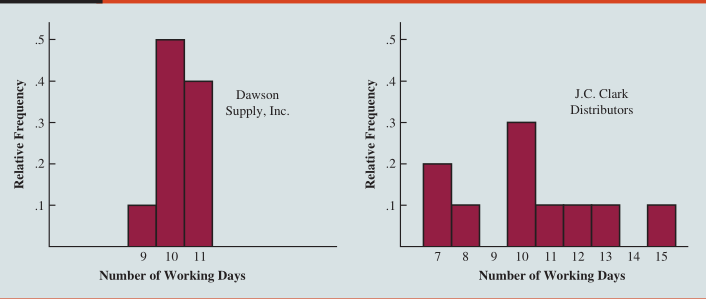
\includegraphics[scale = .4]{Images/variability.png}
     
   \end{figure}

   \item Question - do the two suppliers demonstrate the same degree of reliability in terms of making deliveries on schedule? Note the dispersion, or variability, in delivery times indicated by the histograms. Which supplier would you prefer? The left one right? Why?

\end{itemize}


\end{frame}

\begin{frame}{Range, Interquartile Range and Variance}

\begin{itemize}
   
   \item \citet*{anderson_statistics_2020} discussed three measures of dispersion 

   \begin{itemize}
     \item 1. Range (Largest value  - Smallest Value)
     \item 2. Interquartile Range ($Q_3 - Q_1$)
     \item 3. Sample Variance (or Sample Standard Deviation)
   \end{itemize}

   \item Range is simply the difference between largest and the smallest value. So this is easy to compute. We can use direct Excel functions for it.

   \item Interquartile Range ($Q_3 - Q_1$) is the difference between two quartiles.

   \item And sample variance can be calculated using following formula.

   \begin{align*}
      s^2=\frac{\sum\left(x_i-\bar{x}\right)^2}{n-1}
    \end{align*} 

    \item $s^2$ is the notation for sample variance.

    \item There is another object, called \emph{standard deviation}, which is the square root of the sample variance, so we will write $s$ for standard deviation.

    \item Let's do a simple example using MS-Excel.

\end{itemize}


\end{frame}

\subsection{3. Five-Number Summaries and Boxplots}
\frame{\subsectionpage}

\begin{frame}[allowframebreaks]{Five number Summaries and Boxplot}

\begin{itemize}
  \item We already know the following numerical methods for quantitative variable,

    \begin{itemize}
      \item 1. Smallest value
      \item 2. First quartile $\left(Q_1\right)$
      \item 3. Median $\left(Q_2\right)$
      \item 4. Third quartile $\left(Q_3\right)$
      \item 5. Largest value
    \end{itemize}

    \item A box plot is just a visual representation of these numbers.

    \item Consider following dataset,

    \begin{align*}
      5710 \quad  5755 \quad  5850 \quad  5880 \quad  5880 \quad  5890 \\
       \quad  5920 \quad  5940 \quad  5950 \quad  6050 \quad  6130 \quad  6325
    \end{align*}

  \item The smallest value is 5710 and the largest value is 6325.

  \item We already learned  how to compute the quartiles $\left(Q_1=5857.5 ; Q_2=5905\right.$; and $\left.Q_3=6025\right)$ in Section 3.1. 

  \item Thus, the five-number summary for the monthly starting salary data is

  \begin{align*}
      \text{smallest }= 5710,\quad  Q_1 = 5857.5,\quad  Q_2 = 5905,\quad  Q_3 = 6025,\quad  \text{largest } =6325
  \end{align*}


  \item The five-number summary indicates that the starting salaries in the sample are between 5710 and 6325 and that the median or middle value is 5905 ; and, the first and third quartiles show that \emph{approximately $50 \%$ of the starting salaries are between 5857.5 and 6025}.

  \item Now using this information we can draw a box plot, 


  \begin{figure}
    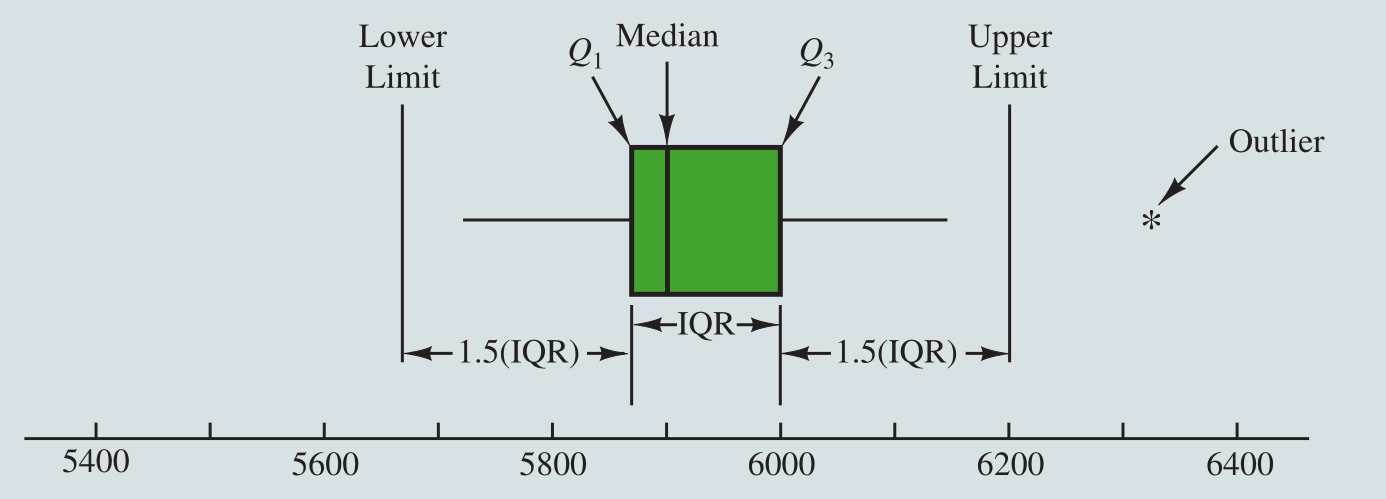
\includegraphics[scale = .25]{Images/Boxplot.png}
  \end{figure}

  \item It is very easy to draw boxplot using Excel, we will do this in the lab class.



\end{itemize}
  
\end{frame}




\begin{frame}{Geometric Mean}

\begin{itemize}

  \item There is another concept known as \emph{Geometric Mean}, which is often used to calculate the \alert{average growth rate}. Here is an example, suppose you invested $100\$$ in a stock and following (see next page) is the yearly return of last $10$ years.

  \item You want to know what is the average annual growth rate of this stock based on this data? This is taken from \citet*{anderson_statistics_2020}

  \item Why we want to calculate average growth rate? Because if you know this then we can predict what will be the value of the stock after next $5$ or $10$ or $15$... years.

  \item For example if the average annual growth rate is $5\%$ or $0.05$, then we can roughly say that the stock's value will be $100(1 + 0.05)^{10}$ after $10$ years (why???).

  \item This is because, 

  \begin{align*}
    \text{after one year } & = 100(1 + 0.05) \\
    \text{after two years } & = 100(1 + 0.05) \times (1 + 0.05) = 100(1 + 0.05)^2   \\
    \vdots\\
    \text{after ten years } & = 100\underbrace{(1 + 0.05) \times (1 + 0.05) \times \ldots \times (1 + 0.05)}_{10} = 100(1 + 0.05)^{10}   \\
  \end{align*}


\end{itemize}
  
\end{frame}



\begin{frame}{Geometric Mean}

\begin{itemize}
\item[]

  \begin{table}
    \begin{align*}
      \begin{array}{cc}
  \text { Year } & \text { Return (\%) } \\
  1 & -22.1 \\
  2 & 28.7 \\
  3 & 10.9 \\
  4 & 4.9 \\
  5 & 15.8 \\
  6 & 5.5 \\
  7 & -37.0 \\
  8 & 26.5 \\
  9 & 15.1 \\
  10 & 2.1
  \end{array}
  \end{align*}
  \end{table}

  \item To calculate the average annual growth rate, we need to first calculate the yearly growth rates.


\end{itemize}
  

\end{frame}



\begin{frame}{Geometric Mean}

\begin{itemize}


  \begin{table}
    \begin{align*}
      \begin{array}{ccr}
\text { Year } & \text { Return (\%) } & \text { Yearly Growth Rate (or Factor) } \\
1 & -22.1 \text{ or } -0.221 & 1 + (-0.221) =   .779 \\
2 & 28.7  \text{ or } 0.287 & 1 + 0.287 = 1.287 \\
3 & 10.9  \text{ or } 0.109 & 1 + .109  = 1.109 \\
4 & 4.9  \text{ or } 0.049 & 1 + 0.049 = 1.049 \\
5 & 15.8  \text{ or } 0.158 & 1 + 0.158 = 1.158 \\
6 & 5.5  \text{ or } 0.055 & 1 + 0.055 = 1.055 \\
7 & -37.0  \text{ or } -0.370 & 1 +(-0.370) = .630 \\
8 & 26.5  \text{ or } 0.265 & 1 + 0.265 = 1.265 \\
9 & 15.1  \text{ or } 0.151 & 1+ 0.151 = 1.151 \\
10 & 2.1  \text{ or } -0.021 & 1+ (- 0.021) = 1.021
\end{array}
    \end{align*}
  \end{table}

  \item In \citet*{anderson_statistics_2020} yearly growth rate is same as Growth Factor.

\end{itemize}
  
\end{frame}



\begin{frame}{Geometric Mean}

\begin{itemize}
  
\item Once we have the yearly growth rate, then we can take the geometric mean of yearly growth rate, and this is calculated as,

\begin{align*}
  &\sqrt[10]{[(.779)(1.287)(1.109)(1.049)(1.158)(1.055)(.630)(1.265)(1.151)(1.021)]} \\
  &= {[(.779)(1.287)(1.109)(1.049)(1.158)(1.055)(.630)(1.265)(1.151)(1.021)]}^{1/10} \\
  &= (1.3344)^{1/10} \\
  &= 1.029 = 1 + 0.029
\end{align*}

\item So $2.9\%$ is the average annual growth rate.



\item If you compare and contrast with Arithmetic mean, then the idea of the Geometric mean is rather than taking sum, we are taking product, and rather than dividing we are taking the power $1/n$ (notice $1/n$ is same as $\sqrt[n]{}$)

\item So the geometric mean is a measure of location that is calculated by finding the $n$th root of the product of $n$ values. The general formula for the geometric mean, denoted $\bar{x}_g$, follows.

$$
\bar{x}_g=\sqrt[n]{\left(x_1\right)\left(x_2\right) \cdots\left(x_n\right)}=\left[\left(x_1\right)\left(x_2\right) \cdots\left(x_n\right)\right]^{1 / n}
$$

\item If you calculate the arithmetic mean of returns from the table, you should get $5.04\%$, and we calculated the geometric mean and we have $2.9\%$.

\item Now we can ask, what might be average return after $10$ years???


\item This problem is taken from \citet*{anderson_statistics_2020} so you should do it on your own.

\end{itemize}
  
\end{frame}





\begin{frame}{Sample Median}


\begin{itemize}

\item The median is another measure of central location. 


\item The median is the value in the \emph{middle} when the data are arranged in \alert{ascending order (smallest value to largest value)}. 


\item With an odd number of observations or samples, the median is the middle value. 


\item With an even number of observations there is no single middle value. In this case, we follow convention and define the median as the average of the values for the middle two observations. So here is how you can find median,


\item Arrange the data in ascending order (smallest value to largest value).
\begin{itemize}

\item (a) For an odd number of observations, the median is the middle value.

\item (b) For an even number of observations, the median is the average of the two middle values.
\end{itemize}

\item Calculating Median by hand is very easy, we will also see an excel in the lab class.

\item Note that median is where the $50\%$ data is on the left and $50\%$ is on the right!



\end{itemize}





\end{frame}


\section{Two Variable Measures For Association : Covariance, Correlation and ScatterPlot}

\subsection{1. Numerical Measures: Covariance and Correlation}
\frame{\subsectionpage}

\begin{frame}[allowframebreaks]{Measure of Association between two variables}{Numerical Measures: Covariance and Correlation}
  
\begin{itemize}
  \item Now we will see some numerical and graphical methods which show association between two variables. The idea here is slightly different than before, here we are interested in \emph{association}...

  \item What do we mean by ``association''? Roughly this means \emph{how two variables behaves together}. 

  \item It's important to mention that \emph{association does not imply causality},... however \emph{causality implies association}.

  \item This means that if the two variables are associated, we cannot say one variable causes the other to change, maybe there is a third variable which causes both of them to move together.

  \item Two important sample \emph{numerical measures are important}, one is \emph{covariance} and other is \emph{correlation}

  \item Here is the formula for covariance


  \begin{align*}
    s_{x, y} = \frac{\sum\left(x_i-\bar{x}\right)\left(y_i-\bar{y}\right)}{n-1}
  \end{align*}

  \item If you do the calculation in excel, then here is how you can do

  \begin{table}[H]
  \centering

\begin{tabular}{|ccc|c|c|c|c|}
\hline & $x_i$ & & $y_i$ & $x_i-\bar{x}$ & $y_i-\bar{y}$ & $\left(x_i-\bar{x}\right)\left(y_i-\bar{y}\right)$ \\
\hline & 2 & & 50 & -1 & -1 & 1 \\
\hline & 5 & & 57 & 2 & 6 & 12 \\
\hline & 1 & & 41 & -2 & -10 & 20 \\
\hline & 3 & & 54 & 0 & 3 & 0 \\
\hline & 4 & & 54 & 1 & 3 & 3 \\
\hline & 1 & & 38 & -2 & -13 & 26 \\
\hline & 5 & & 63 & 2 & 12 & 24 \\
\hline & 3 & & 48 & 0 & -3 & 0 \\
\hline & 4 & & 59 & 1 & 8 & 8 \\
\hline & 2 & & 46 & -1 & -5 & 5 \\
\hline Totals & $\overline{30}$ & & $\overline{510}$ & 0 & 0 & 99 \\
\hline
\end{tabular}

\item and then the covariance is 

  \begin{align*}
    s_{x, y} = \frac{\sum\left(x_i-\bar{x}\right)\left(y_i-\bar{y}\right)}{n-1} = \frac{99}{10-1} = 11
  \end{align*}

\item Now how do we interpret the covariance? The idea is \emph{positive covariance means positive association, this happens when both deviations are either positive or negative}, and similarly, \emph{negative covariance means negative association, and this happens when one deviation is positive and other is negative}



    
  \end{table}


  \item We will see some applications in Excel, 


\framebreak

\item The formula for correlation is just a modification of the covariance formula, but here we just need standard deviation of each of the variables, so here are the covariance of $x$ and $y$ and standard deviation of $x$ and $y$ respectively

\begin{align*}
s_{x, y} & =\frac{\sum\left(x_i-\bar{x}\right)\left(y_i-\bar{y}\right)}{n-1} \\
s_x & =\sqrt{\frac{\sum\left(x_i-\bar{x}\right)^2}{n-1}} \\
s_y & =\sqrt{\frac{\sum\left(y_i-\bar{y}\right)^2}{n-1}}
\end{align*}


\item The correlation formula is the following,

\begin{align*}
  r_{x, y}=\frac{s_{x , y}}{s_x s_y}
\end{align*}


\item Interestingly the correlation between $x$ and $y$, which we denoted with $r_{x y}$ will always lie between $-1$ and $1$, so 

\begin{align*}
  -1 \leq r_{x, y} \leq 1
\end{align*}

\item Interpretation is similar to covariance, however here we can also understand the strength of the association. 

\item If the value of $r_{x, y}$ is \alert{close to $1$ indicates strong positive correlation}, which means strong positive association between two variables, 

\item Similarly  if the value of $r_{x, y}$ is \alert{close to $-1$ indicates strong negative correlation}, which means strong positive association between two variables, 

\item And finally if the value is close to $0$ indicates, zero correlation and there is no association.


\end{itemize}


\end{frame}


\subsection{2. Graphical Measure: Scatterplot}
\frame{\subsectionpage}

\begin{frame}[allowframebreaks]{Measure of Association between two variables}{Graphical Measures: Scatterplot}
  
\begin{itemize}

\item scatterplot is a plot where we plot $(x,y)$ pairs in the $(x-y)$ co-ordinate, for example here is a data, which has two variables, the number of commercials which is $x$ and sales (in 100\$) which is $y$


\begin{table}[H]
\centering
  \begin{tabular}{c|c|c} 
Week & Number of Commercials $\boldsymbol{x}$ & Sales Volume (\$100s) $\boldsymbol{y}$ \\
1 & 2 & 50 \\
2 & 5 & 57 \\
3 & 1 & 41 \\
4 & 3 & 54 \\
5 & 4 & 54 \\
6 & 1 & 38 \\
7 & 5 & 63 \\
8 & 3 & 48 \\
9 & 4 & 59 \\
10 & 2 & 46
\end{tabular}
\end{table}

we can plot the $(x, y)$ pairs as follows, 

\framebreak

\begin{figure}[H]
\centering
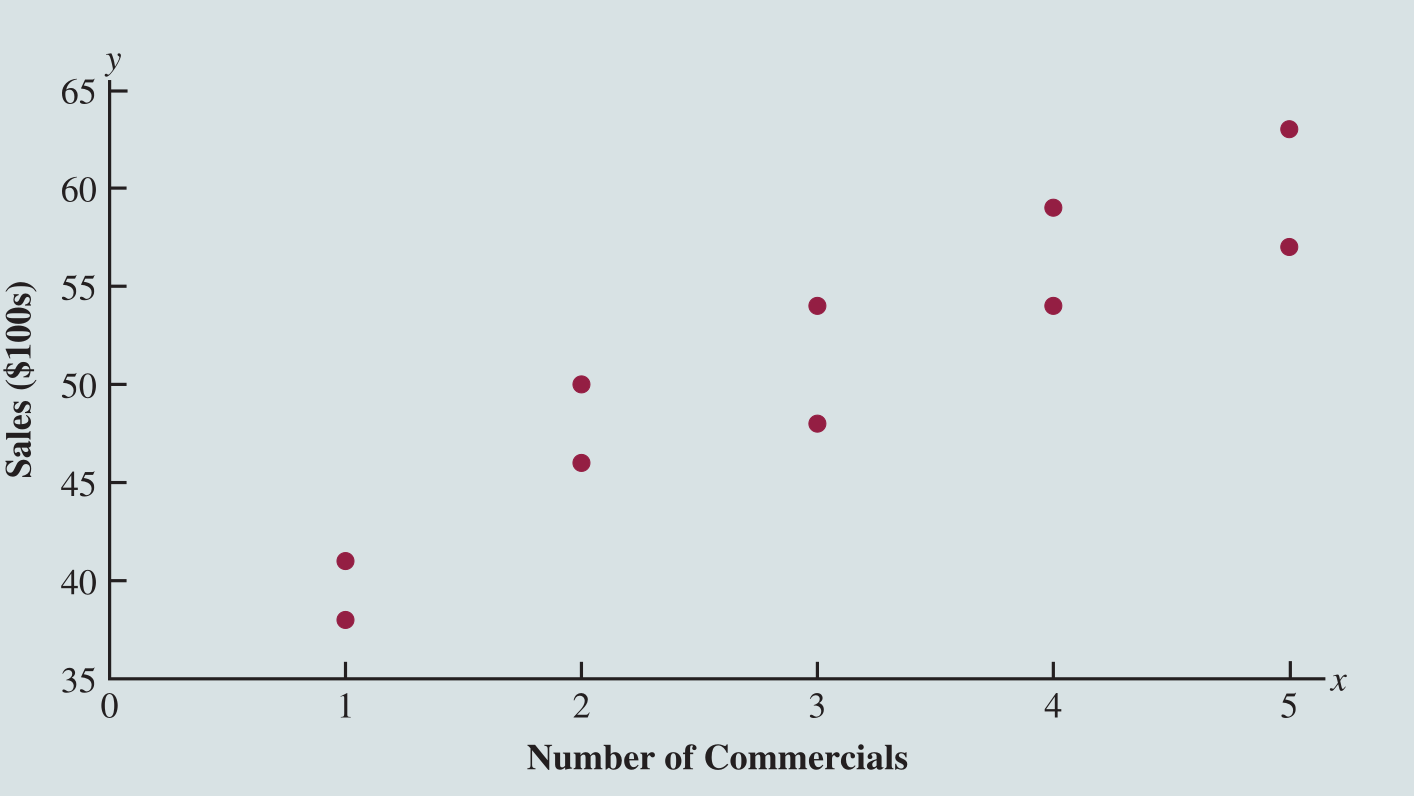
\includegraphics[scale = .25]{Images/scatter_plots.png}
\caption{Scatter plot between $x$ and $y$}
\end{figure}

\item We will usually use MS-Excel to produce the scatter plot, and it's quite easy using Excel. 



\framebreak

\item It's important to note that, scatter-plot also shows positive and negative association, following picture is useful to understand this,

\begin{figure}[H]
\centering
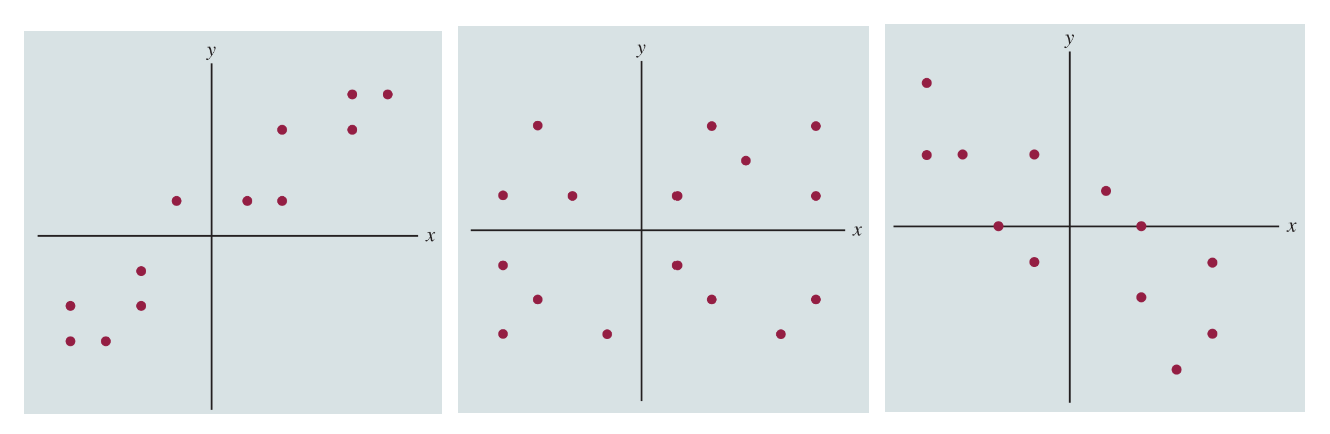
\includegraphics[scale = .30]{Images/scatterplots.png}
\caption{On the \emph{Left}: \alert{Positive Association}, On the \emph{Middle}: Almost \alert{No Association}, and On the \emph{Right}: \alert{Negative Association}}
\end{figure}

\item The easy way to remember this is to notice - \emph{when $x$ is increases whether $y$ increases or decreases...}


\item Clearly on the picture, on the left if we calculate $r_{x, y}$ it should be close to $1$, on the middle it should be close $0$ and on the right it should be close to $-1$


\end{itemize}


\end{frame}


\section{Chapter Recap For the Descriptive Statistics Part}
\frame{\sectionpage}

\begin{frame}[allowframebreaks]{ Recap For the Descriptive Statistics Part}
  

\begin{itemize}
  \item Since we have learned a lot of things it's a good idea to make a list of what we have learned in The Descriptive Statistics part,

  \item Here is what we have learned in the Tabular and Graphical Side

  \begin{itemize}
    \item  Frequency Distribution Table, Bar Chart and Pie Chart
    \item Grouped Frequency Distribution Table and Histogram 
    \item Cross-tabulation or Contingency Table or Joint Frequency Distribution, and Side-by-Side Bar Chart or Stacked Bar Chart 
    \item Bivariate Frequency Distribution Table and Joint Histogram 
    \item Scatter Plot For Association
    \item Boxplot

  \end{itemize}

  \framebreaks

    \item Here is what we have learned in the Numerical Side
  \begin{itemize}
    \item Mean, Weighted Mean, Percentile (Quantile), Median and Mode
    \item Largest Value, Smallest Value, Range, Interquartile Range, Variance
    \item Covariance and Correlation 

    \item You should know the excel functions of the numerical measures...
  \end{itemize}


\end{itemize}

\end{frame}


\begin{frame}[allowframebreaks]{References}
 \vspace*{.3cm} 

\scriptsize
 % \printbibliography[maxnames=99]

  % \nocite{*}
  \bibliographystyle{apalike}
  \bibliography{../common/references}  
  % \nocite{*}
  
\end{frame}

\end{document}
